The purpose of this test is to test the observer based LQR (OBLQR) controller on the Hi-Fi simulation. Focus will be on how the cargo hold air temperature and evaporator output refrigerant temperature reacts, when the model is near the operating point and when different disturbances are applied. Additionally, the energy consumption for the actuators of the observer based controller will be compared to the energy consumption for the actuators of the PID controller.

\subsection{Test framework}
When the HiFi simulation model is initialized, the system takes approximately 1.5 hours until it converges to steady state. Since the OBLQR controller is not expected to work well when operating far from the linearisation point, the existing PID control structure is used to handle the initial transient behavior. This is done as not all of the states in the Hi-Fi simulation model are available. Thus, they can not be initialised at the operating point, and in stead the PID controller is used to bring the system \textbf{near} the operating point before the OBLQR controller can be applied. 
As the simulation model is deterministic, it is possible to choose a fixed time when the OBLQR controller can take over, and then know that the system is some fixed distance from the operating point. This is used to show whether the OBLQR controller can handle deviations from the operating point.

\begin{figure}[h!]
	\centering
	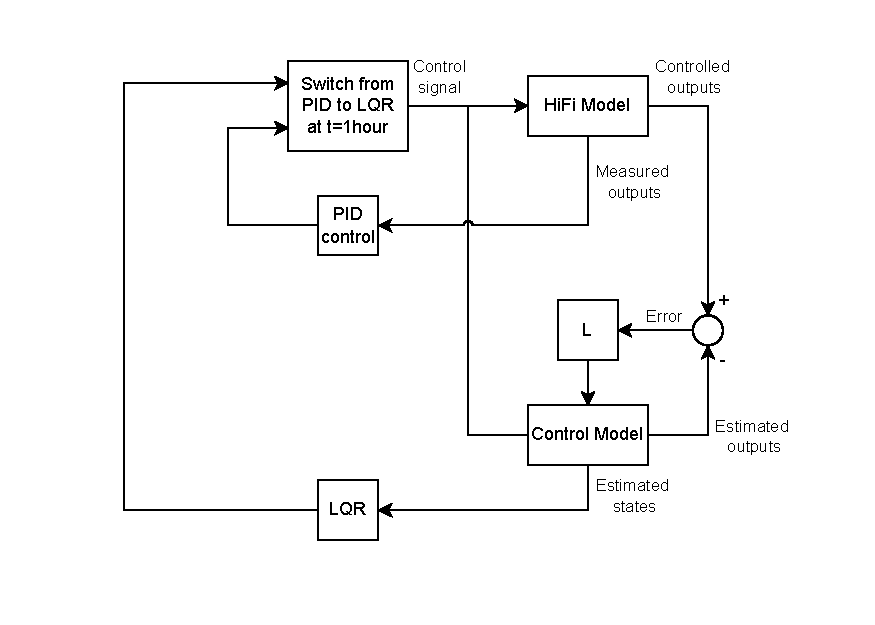
\includegraphics[width=0.8\textwidth]{Graphics/HiFi_simulation_test_diagram.pdf}
	\caption{Top: Cargo hold air temperature. $T_0$ = -4.25$^{\circ}$C. Bottom: Evaporator vapor refrigerant temperature. $T_0$ = -5.55$^{\circ}$C}
	\label{fig:test_setup}
\end{figure}

The test setup is sketched in \cref{fig:test_setup}. A switch is inserted in the simulation which changes the inputs to the Hi-Fi simulation from the PID control structure to the LQR controller at some specified time. It takes two inputs: the vector of the PID chosen control inputs and the vector of the OBLQR controller input. The PID control structure inputs are fed to the system until the time reaches 1 hour, at which point the states will be \textbf{near} the linearisation point. At this point, the switch selects the OBLQR control inputs to be fed to the system. Until the switching time, the control model (observer) states are forced to stay at 0.

Two simulations will run in parallel: The above described, and one where the PID control structure continues to regulate the system for the entire simulation. This allows for comparison between the two control strategies.\\

Three scenarios are simulated:

\begin{enumerate}
	\item No disturbance (at operating point)
	\item Sine wave disturbance
	\item Step away from operating point disturbance
\end{enumerate}

\noindent For each of the three scenarios the two outputs, namely the cargo hold air temperature and evaporator output refrigerant temperature are plotted along with the controller inputs. The two outputs are plotted from both the Hi-Fi simulation and the observer to see whether the observer successfully estimates those two states. Furthermore the output of the Hi-Fi model is plotted when its own PID controller structure inputs are fed to it to benchmark it against the LQR controller. Lastly the average power consumption by the two control strategies are mentioned to evaluate the efficiency of the OBLQR.

\subsection{Tuned OBLQR controller: Constant disturbance}
This test illustrates the performance of the OBLQR controller in the best case scenario, namely where the disturbance (ambient temperature) is held constant at 20$^{\circ}$C. This is the operating point for the disturbance. The controlled outputs are seen in \cref{fig:LQR_wellTuned_noDist}. The OBLQR controller is set to start regulating the system at time $t=1$ hours, at which point it will attempt to drive the states to 0. This is done to illustrate whether the OBLQR controller can drive the states to zero, when initialised outside the operating point.

\begin{figure}[H]
	\centering
	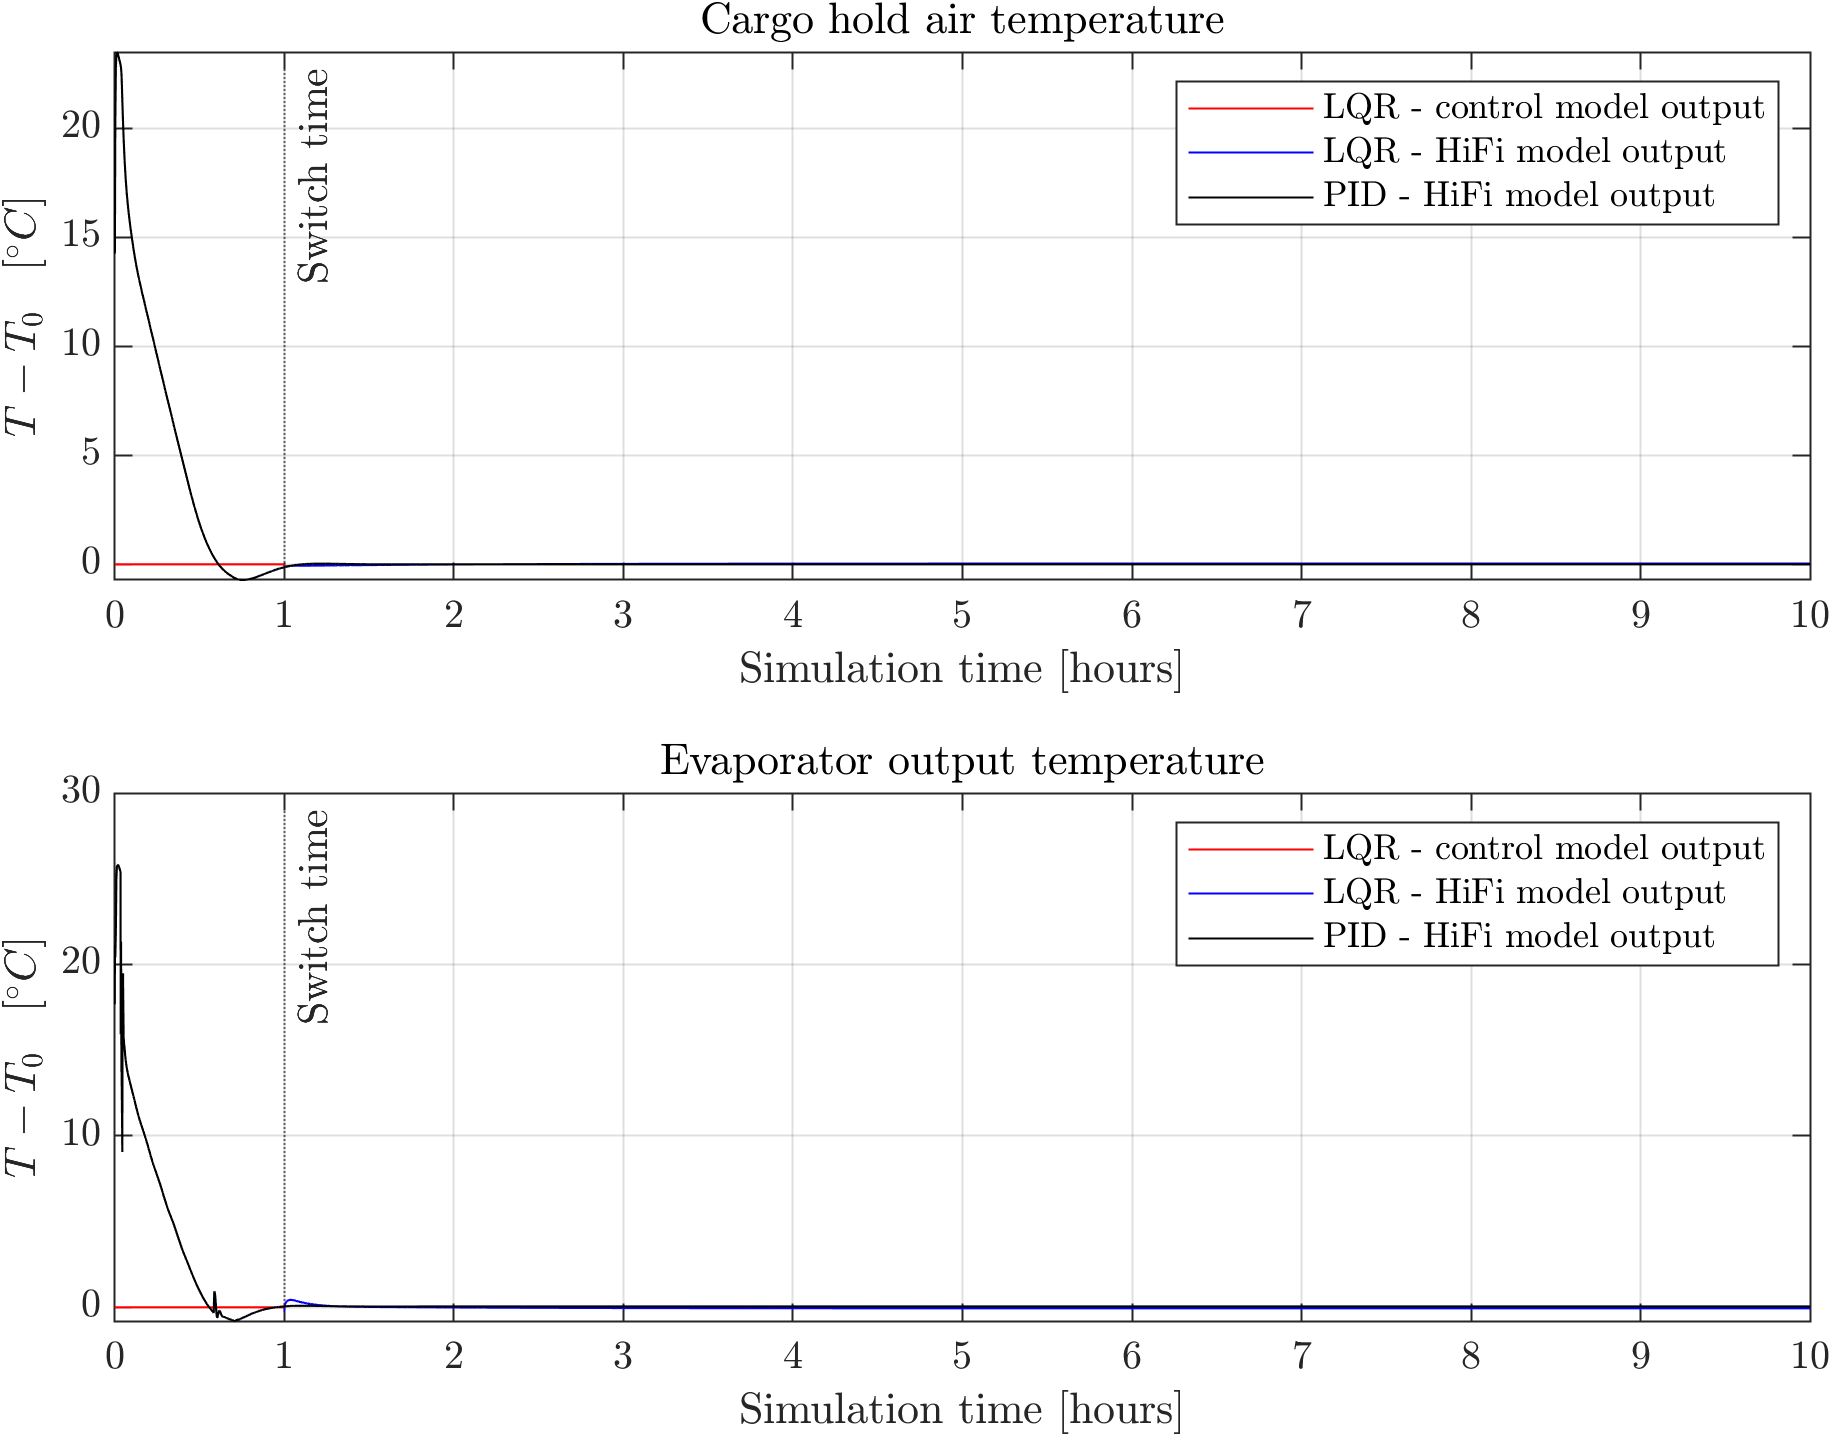
\includegraphics[width=0.8\textwidth]{Graphics/fig_LQRvsKresten_noDist.png}
	\caption{No disturbance case: Top: Cargo hold air temperature. $T_0$ = -4.25$^{\circ}$C. Bottom: Evaporator vapor refridgerant temperature. $T_0$ = -5.55$^{\circ}$C. The controlled outputs from both controllers are regulated near zero}
	\label{fig:LQR_wellTuned_noDist}
\end{figure} 
The controlled outputs of the OBLQR controller is regulated to near zero, and as such, the controller seem to work near the linearisation point. This also implies that the observed states are accurate. The "LQR - control model outputs", are the observer estimates of the outputs. The observer estimates can not be distinguished from the "LQR - HiFi model output" which is the actual outputs of the HiFi model. To further investigate the accuracy of the controlled outputs, a zoomed version of \cref{fig:LQR_wellTuned_noDist} is consulted in \cref{fig:LQR_wellTuned_noDist_zoom}.


\begin{figure}[H]
	\centering
	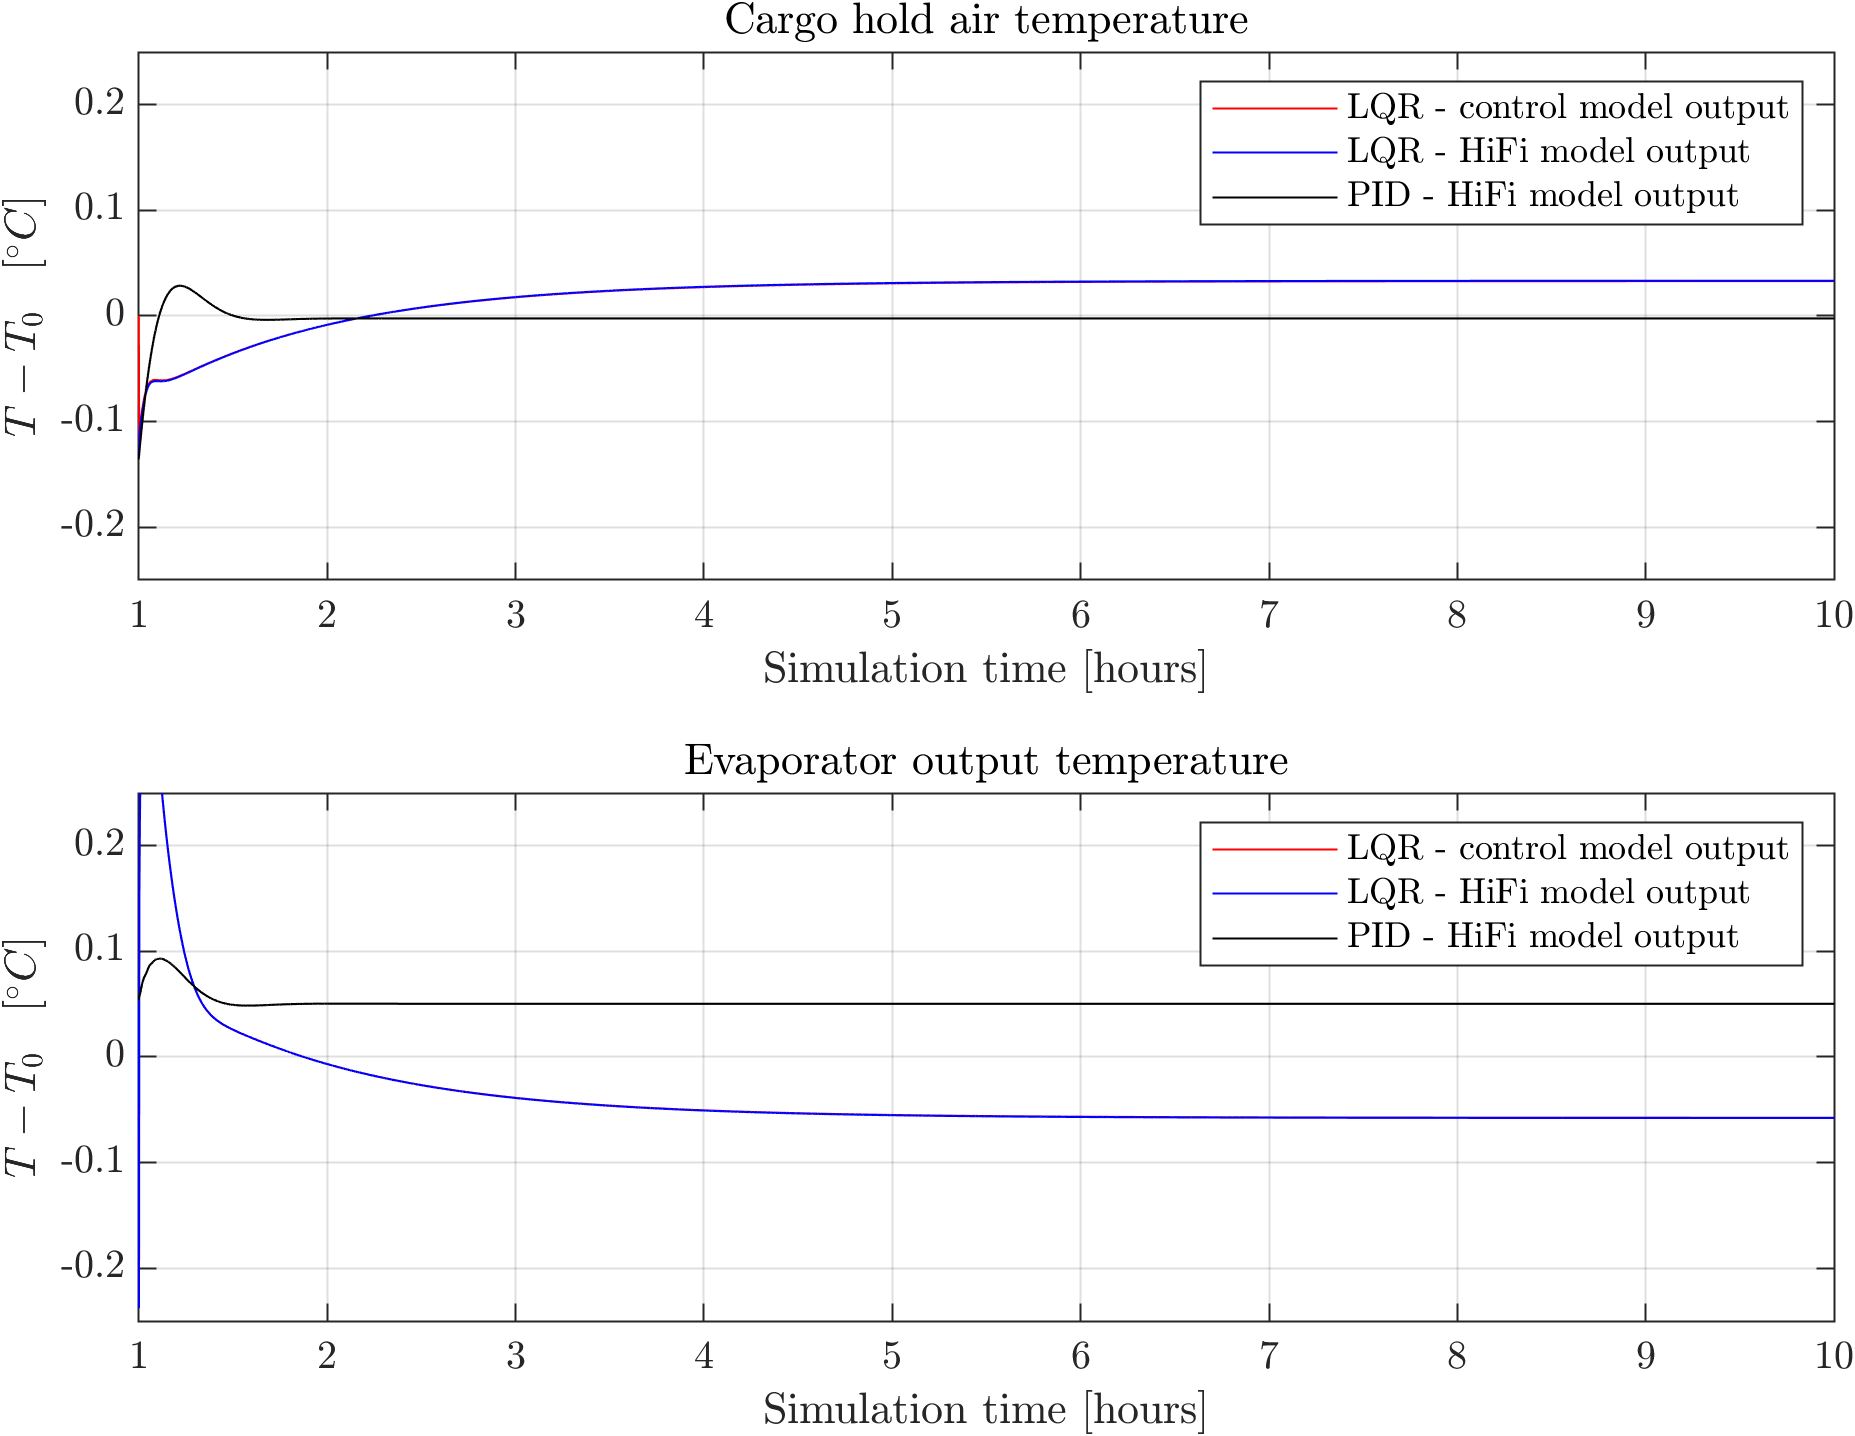
\includegraphics[width=0.8\textwidth]{Graphics/fig_LQRvsKresten_noDist_zoom.png}
	\caption{Zoomed version of \cref{fig:LQR_wellTuned_noDist}. No disturbance case: Top: Cargo hold air temperature. $T_0$ = -4.25$^{\circ}$C. Bottom: Evaporator vapor refridgerant temperature. $T_0$ = -5.55$^{\circ}$C. The OBLQR has a slight steady state error of about 0.03 $^{\circ}$C in the first subplot. In the second subplot it is -0.06 $^{\circ}$C. The settling time is longer for both cases than that of the PID controller}
	\label{fig:LQR_wellTuned_noDist_zoom}
\end{figure}

\noindent The error is so numerically small (0.02$^{\circ}$C for cargo temperature and 0.06 $^{\circ}$C evaporator output refrigerant temperature) that most real temperature sensors would be unable to detect it. The LQR controller is thus shown to be able to drive the system to practically zero, when no disturbance is present. The settling time is however noticeably longer than that of the PID controlled system. 

The control inputs during this test is seen in \cref{fig:inputs_noDist}. As expected the removed inputs are constant at the operating point, but perhaps less expected the remaining inputs $\Theta_1$ and $U_{fan2}$ do not change despite the air and evaporator output error.

\begin{figure}[H]
	\centering
	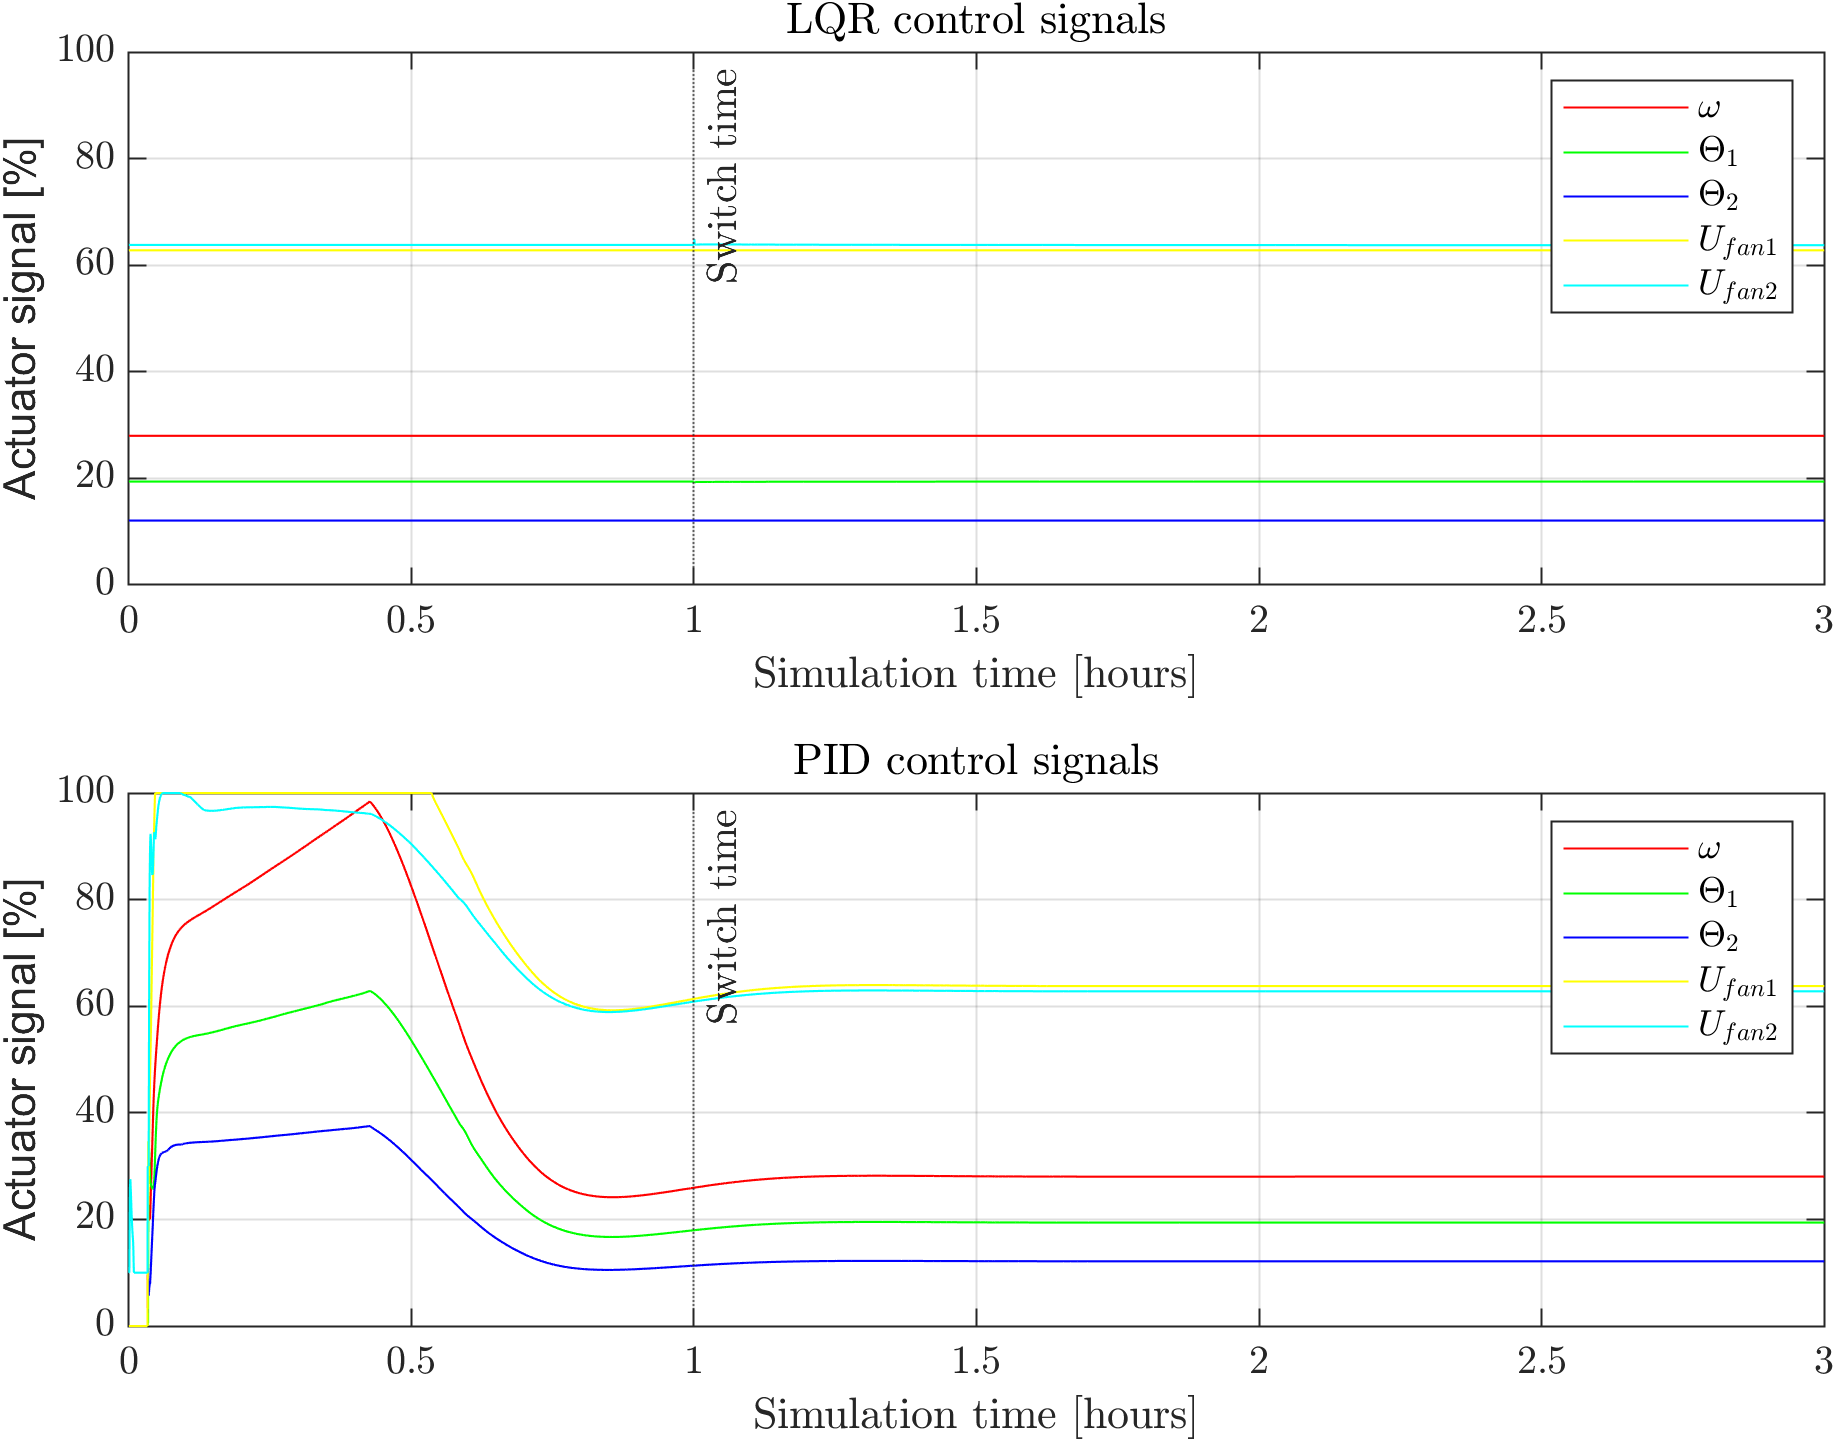
\includegraphics[width=0.8\textwidth]{Graphics/fig_inputs_noDist.png}
	\caption{No disturbance case: Plot of the control signals applied to the Hi-Fi Simulation. Top: LQR control signals. Bottom: Hi-Fi simulation PID control signals.}
	\label{fig:inputs_noDist}
\end{figure}
All of the control signals are within the interval of 0 to 100, and are thus valid. The fact that the OBLQR control signals $ \Theta_1, U_{fan2} $ seem to be constant is a bit surprising. It is therefore investigated closer by a zoomed plot in \cref{fig:inputs_noDist_zoom}.

\begin{figure}[H]
	\centering
	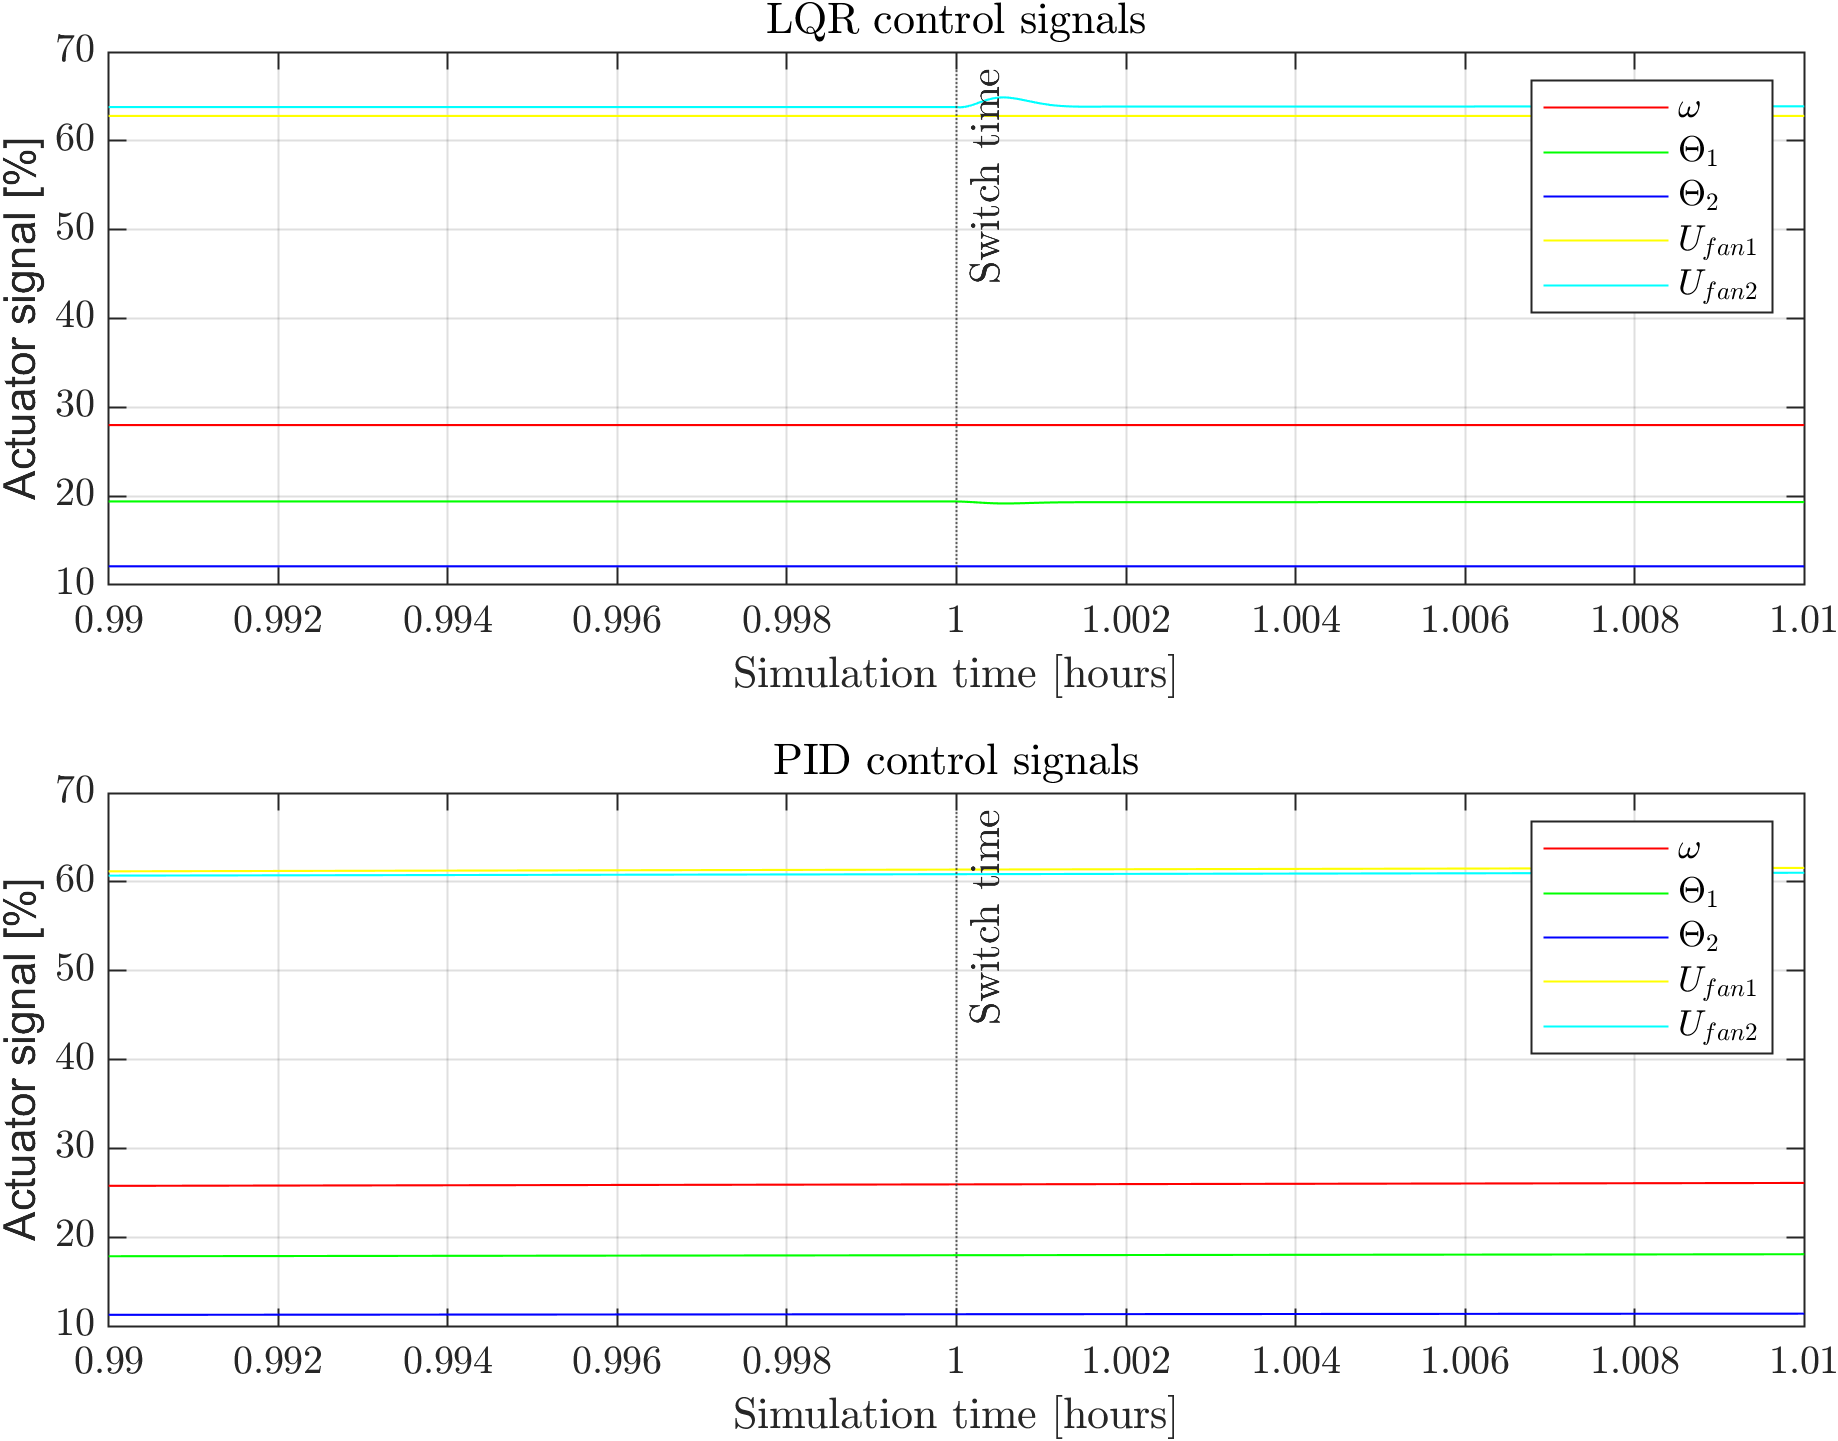
\includegraphics[width=0.8\textwidth]{Graphics/fig_inputs_noDist_zoom.png}
	\caption{Zoomed version of \cref{fig:inputs_noDist}. No disturbance case: Plot of the control signals applied to the Hi-Fi Simulation (zoomed). Top: LQR control signals. Bottom: Hi-Fi simulation PID control signals.}
	\label{fig:inputs_noDist_zoom}
\end{figure}
 
In \cref{fig:inputs_noDist_zoom}, it can be seen that $ \Theta_1, U_{fan2} $ are in fact varying slightly to, just after the switch time. This confirms that the controller is reacting to the controlled outputs. \\
\noindent As the linearised model of the OBLQR model is based on the same linearisation point as the steady state PID controllers, the power consumptions are very similiar at 1.67 \si{kW} and 1.67 \si{kW} for respectively the OBLQR controller and the PID controller. The energy consumption throughout the entire test case is 25.22 \si{kWh} for the OBLQR, compared with 25.14 \si{kWh} for the PID controller. Thus for a nominal case, the OBLQR controller does not provide better energy efficiency than the PID controller. A possible reason the OBLQR is not better than the PID controller is a combination of two elements. Firstly, as described in \cref{sec:model-verification} and \cref{sec:mod_lin} the modeling of the system had some mismatches that meant that parts of the system were disconnected in the model. As a result, 3 of the inputs ($\omega$, $U_{fan_1}$ and $\theta_2$) did not map to the states of the model. These inaccuracies meant that the linearisation had to rely on the PID controller and the HiFi model for obtaining the linearisation point. Thus the 3 control inputs that did not map to the states are held constant at the same values as the steadu state values of the PID controller in the nominal case, as seen in \cref{fig:inputs_noDist}. Secondly, as a direct result of the mismatches, the accuracy of the obtained model did not allow for possible improvements in terms of varying the combinations of inputs that could bring the system to the same outputs but with less power required. 


\newpage
\subsection{Tuned OBLQR controller: Sine disturbance}
The controllers dynamic performance is now investigated as a sine disturbance is applied to the system. As before, the PID controller will handle the initial hour of settling. The LQR then starts regulating the system, and at time $t=3$ hours, the disturbance is injected to the ambient temperature. The disturbance is a sine wave with an amplitude of 5$^{\circ}$C and a period of 10 minutes. The controlled outputs are seen in \cref{fig:LQR_wellTuned_sineDist}.

\begin{figure}[H]
	\centering
	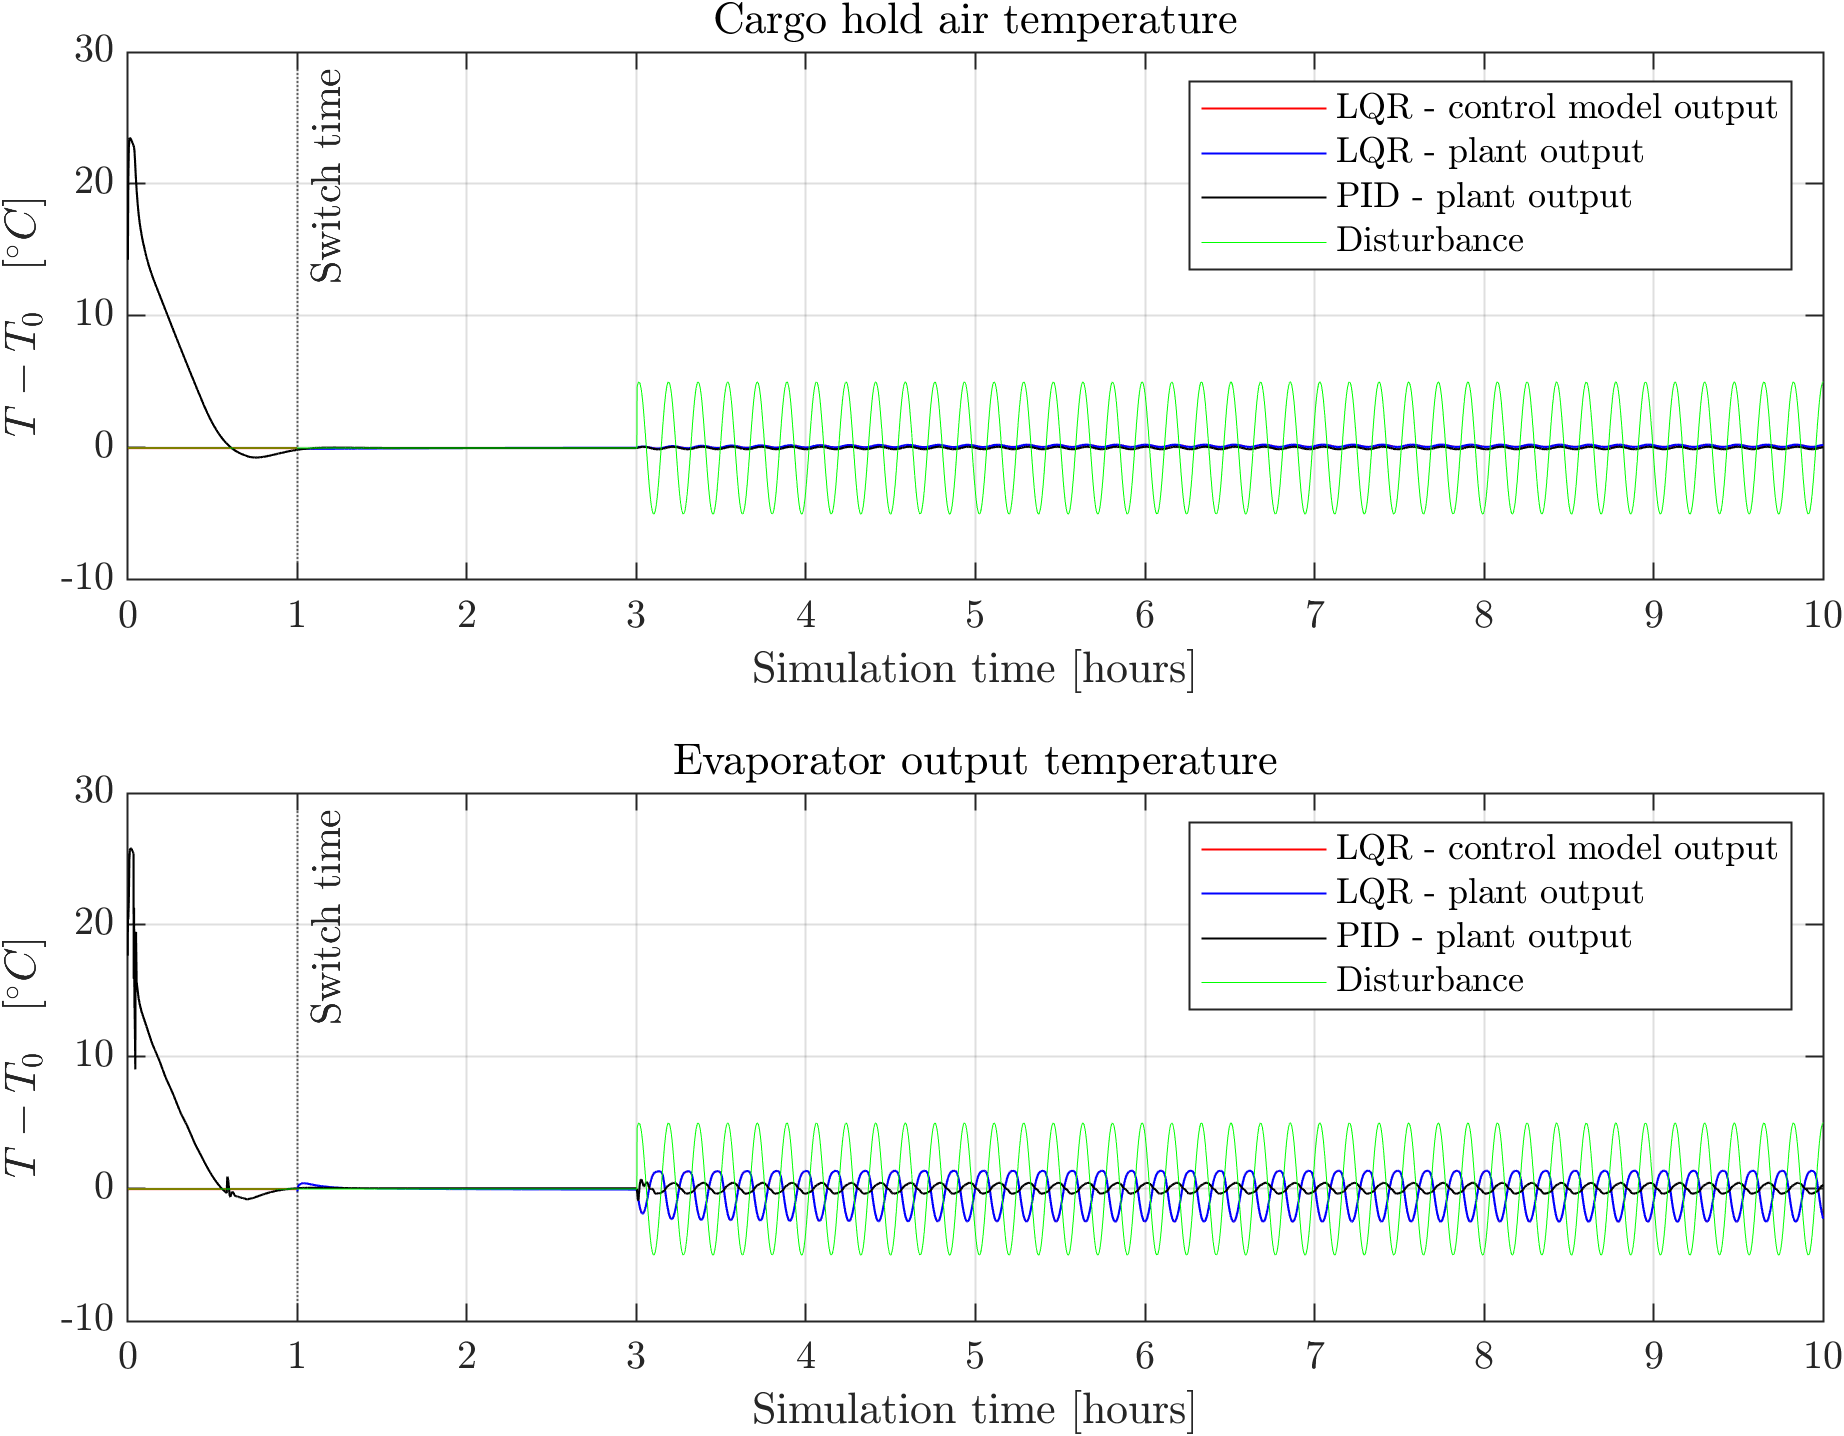
\includegraphics[width=0.8\textwidth]{Graphics/fig_LQRvsKresten_sineDist.png}
	\caption{Sine disturbance case: Top: Cargo hold air temperature. $T_0$ = -4.25$^{\circ}$C. Bottom: Evaporator vapor refridgerant temperature. $T_0$ = -5.55$^{\circ}$C}
	\label{fig:LQR_wellTuned_sineDist}
\end{figure}

\noindent When inspecting the controlled outputs for the two controllers in \cref{fig:LQR_wellTuned_sineDist}, the cargo hold temperature in subplot 1 is hard to judge, and a zoomed plot is required as in \cref{fig:LQR_wellTuned_sineDist_zoom}. Referring to subplot 2, the evaporator output temperature seem to be better controlled by the PID controller than the OBLQR controller, however, a closer look is required as well. \cref{fig:LQR_wellTuned_sineDist_zoom} shows a zoomed in version of \cref{fig:LQR_wellTuned_sineDist}, where the steady state behavior of the two outputs is seen.

\begin{figure}[H]
	\centering
	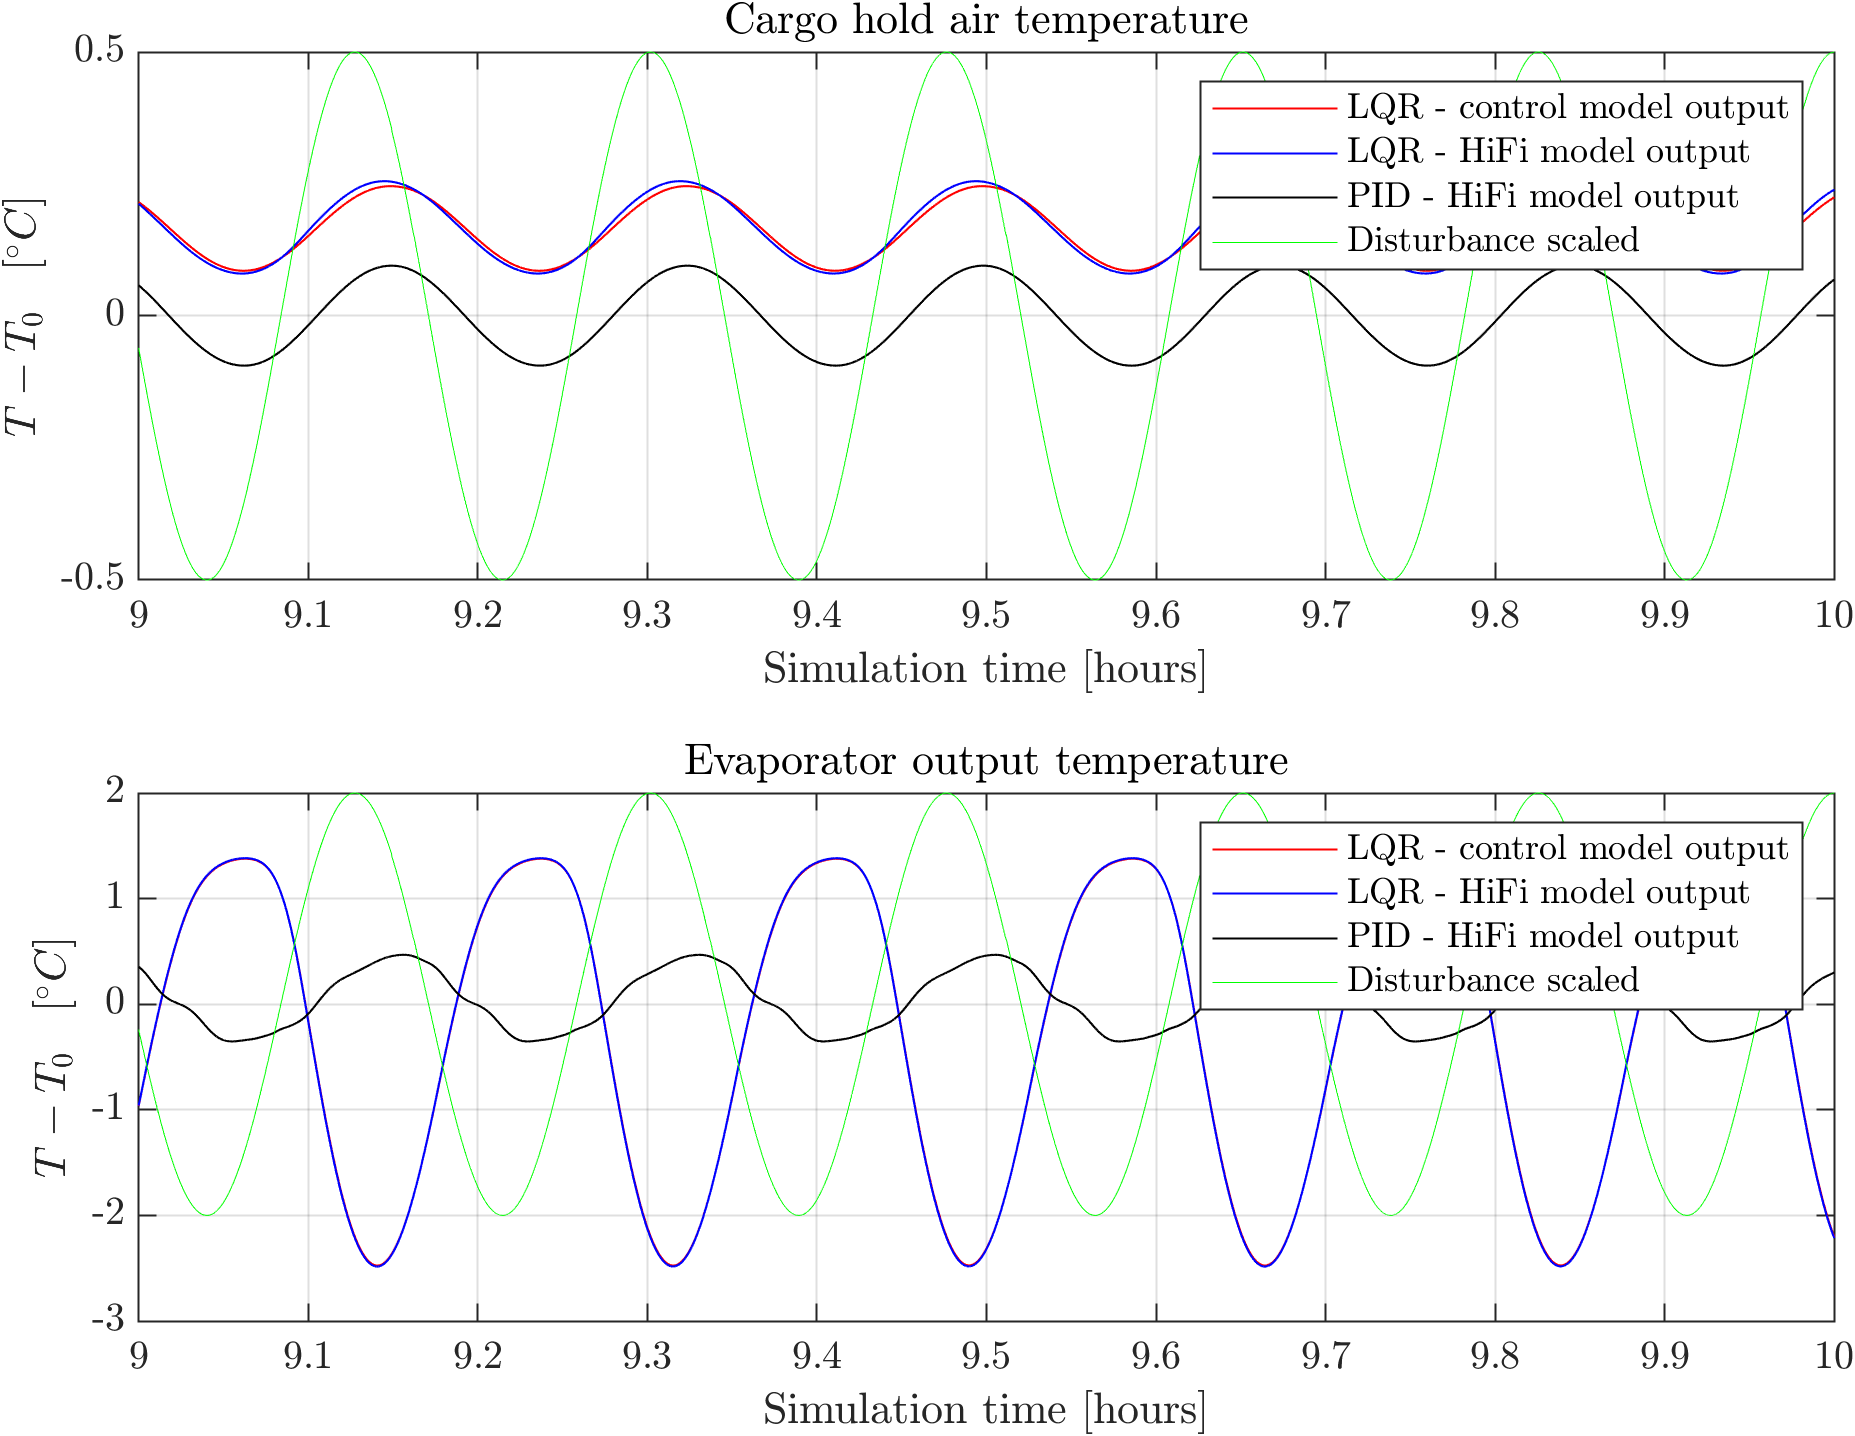
\includegraphics[width=0.8\textwidth]{Graphics/fig_LQRvsKresten_sineDist_zoom.png}
	\caption{Zoomed version of \cref{fig:LQR_wellTuned_sineDist}. Sine disturbance case: Top: Cargo hold air temperature. $T_0$ = -4.25$^{\circ}$C. Bottom: Evaporator vapor refrigerant temperature. $T_0$ = -5.55$^{\circ}$C}
	\label{fig:LQR_wellTuned_sineDist_zoom}
\end{figure}

\noindent A few interesting things are revealed in these plots. 
Firstly, the amplitude of the oscillations on the cargo hold air temperature are not visibly different for the two control strategies. The amplitude of the oscillation is 0.18$^{\circ}$C. Thus the OBLQR control strategy is performing well at minimizing oscillating ambient temperatures effect on the air temperature inside the trailer. However the OBLQR controller has an offset of about 0.15 $ ^{\circ} $C, compared with no offset of the PID controller. The PID controller is thus considered better than OBLQR for handling oscillating disturbances.

Secondly, the amplitude of the oscillations of $T_v$ are considerably lower with the PID control structure, than with the LQR controller. This implies that the OBLQR is less efficient in correcting errors on that particular state. Intuitively this would be improved by penalizing the relevant entry in the $Q$ weighing matrix. This has been attempted, and it was found that increasing the weight led to larger oscillations in the state. The PID controller is thus considered better at controlling the evaporator superheat than the OBLQR. \\

It is likely that the main cause of the poorer performance, is the control model itself. Due to the simplifications made and described in \cref{sec:model-verification} and \cref{sec:mod_lin}, information about the unused inputs' ($\omega$, $U_{fan_1}$ and $\theta_2$) effect on the states was lost. It is expected that a controller (such as the PID structure), that is able to regulate these inputs would perform better, i.e. minimize the oscillations. This is further confirmed when looking at the inputs from the two different control structures in \cref{fig:inputs_sineDist} and \cref{fig:inputs_sineDist_zoom}. As expected the PID control structure utilizes all control inputs to minimize the disturbances effect on the system. As seen in the below figures, all of the control signals are inside the valid interval from 0 to 100.\\

\begin{figure}[H]
	\centering
	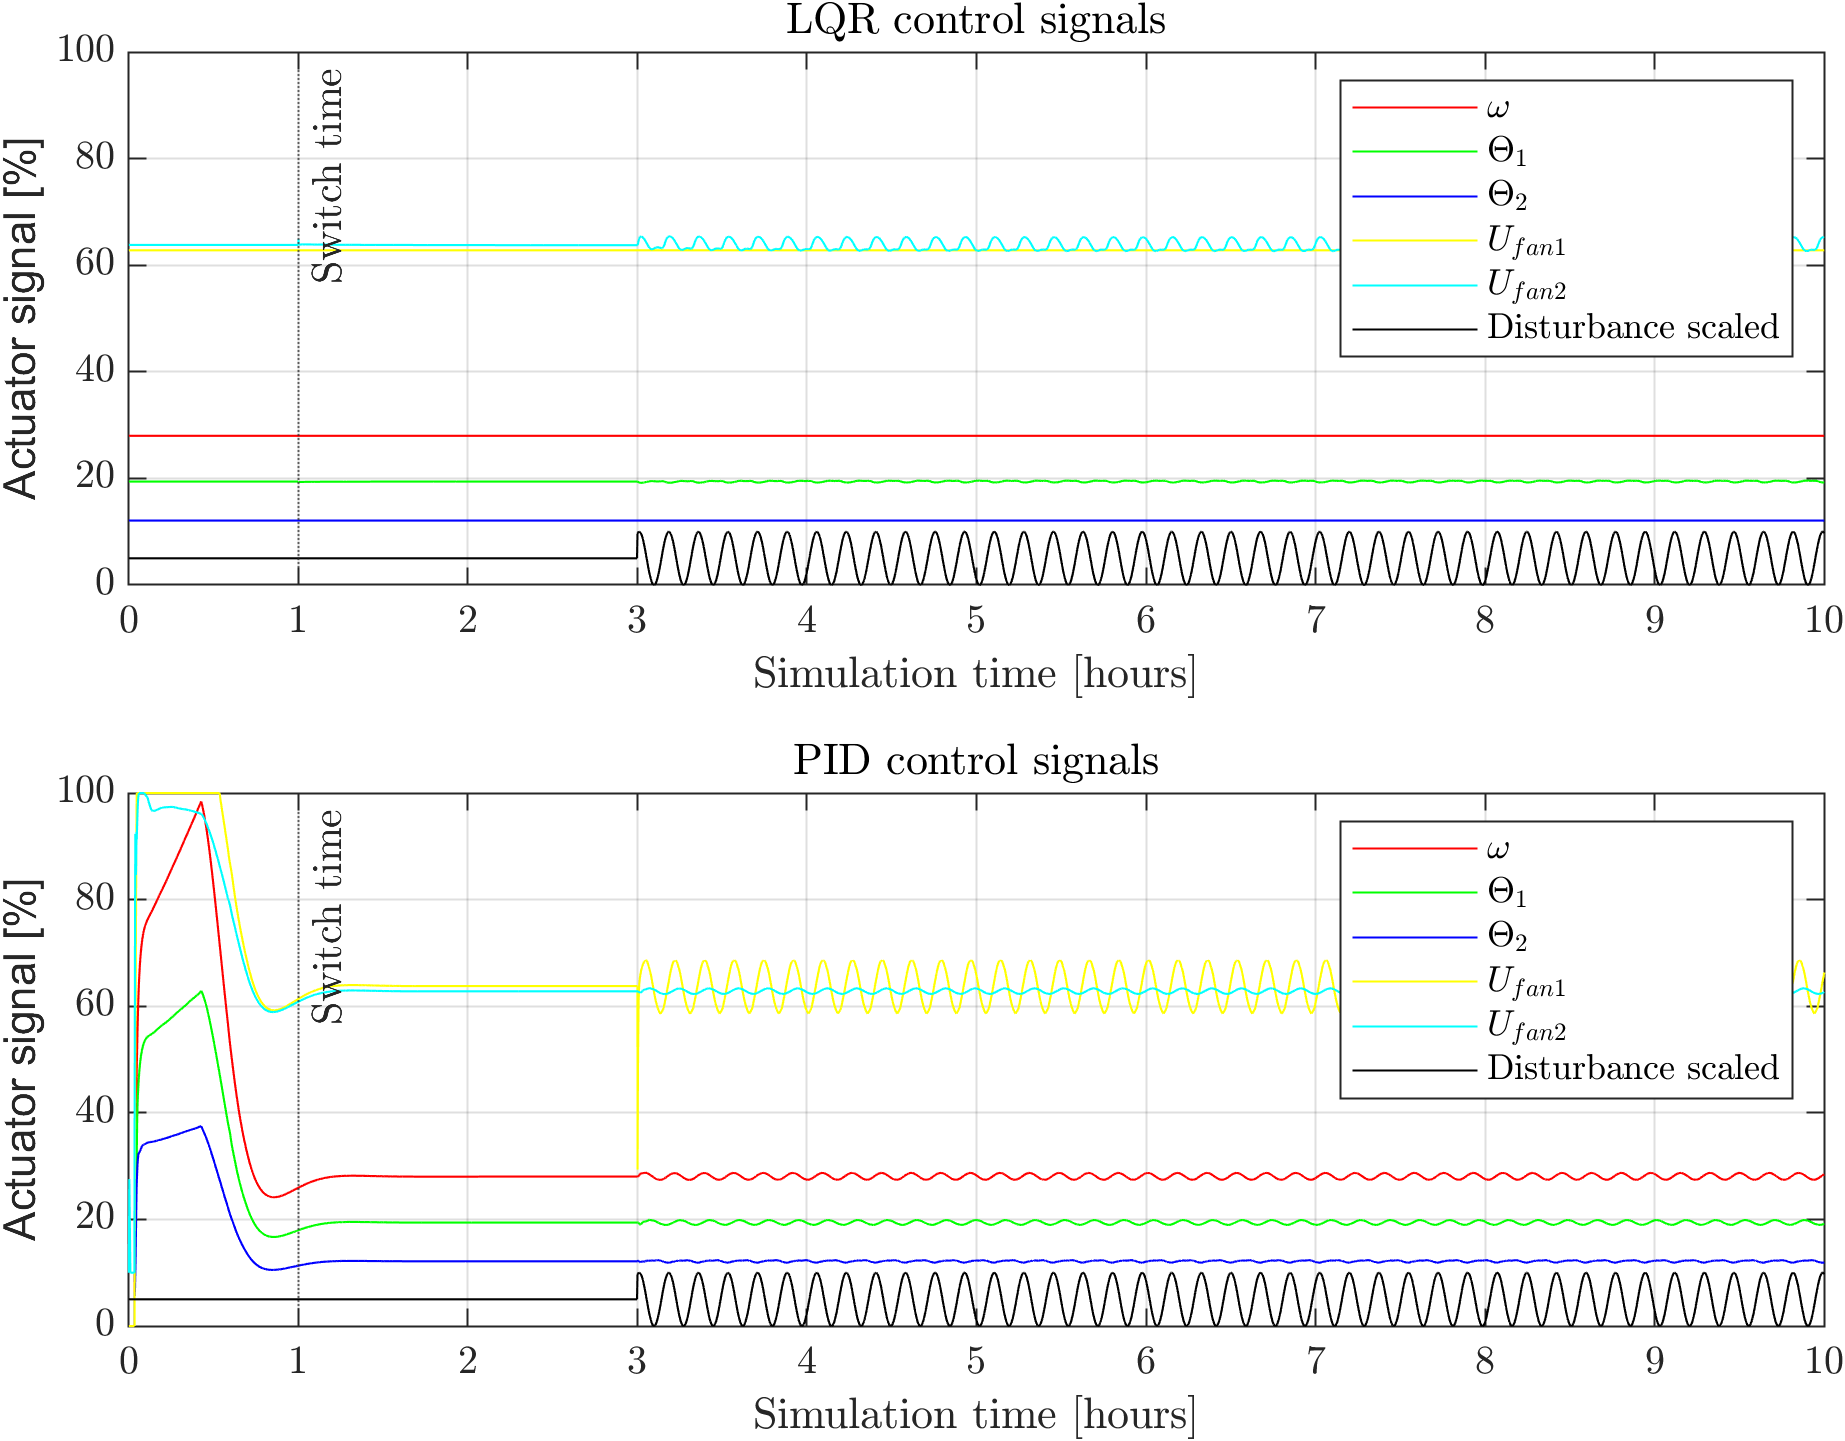
\includegraphics[width=0.71\textwidth]{Graphics/fig_inputs_sineDist.png}
	\caption{Sine disturbance case: Plot of the control signals applied to the Hi-Fi Simulation. Top: LQR control signals. Bottom: Hi-Fi simulation PID control signals.}
	\label{fig:inputs_sineDist}
\end{figure}

\begin{figure}[H]
	\centering
	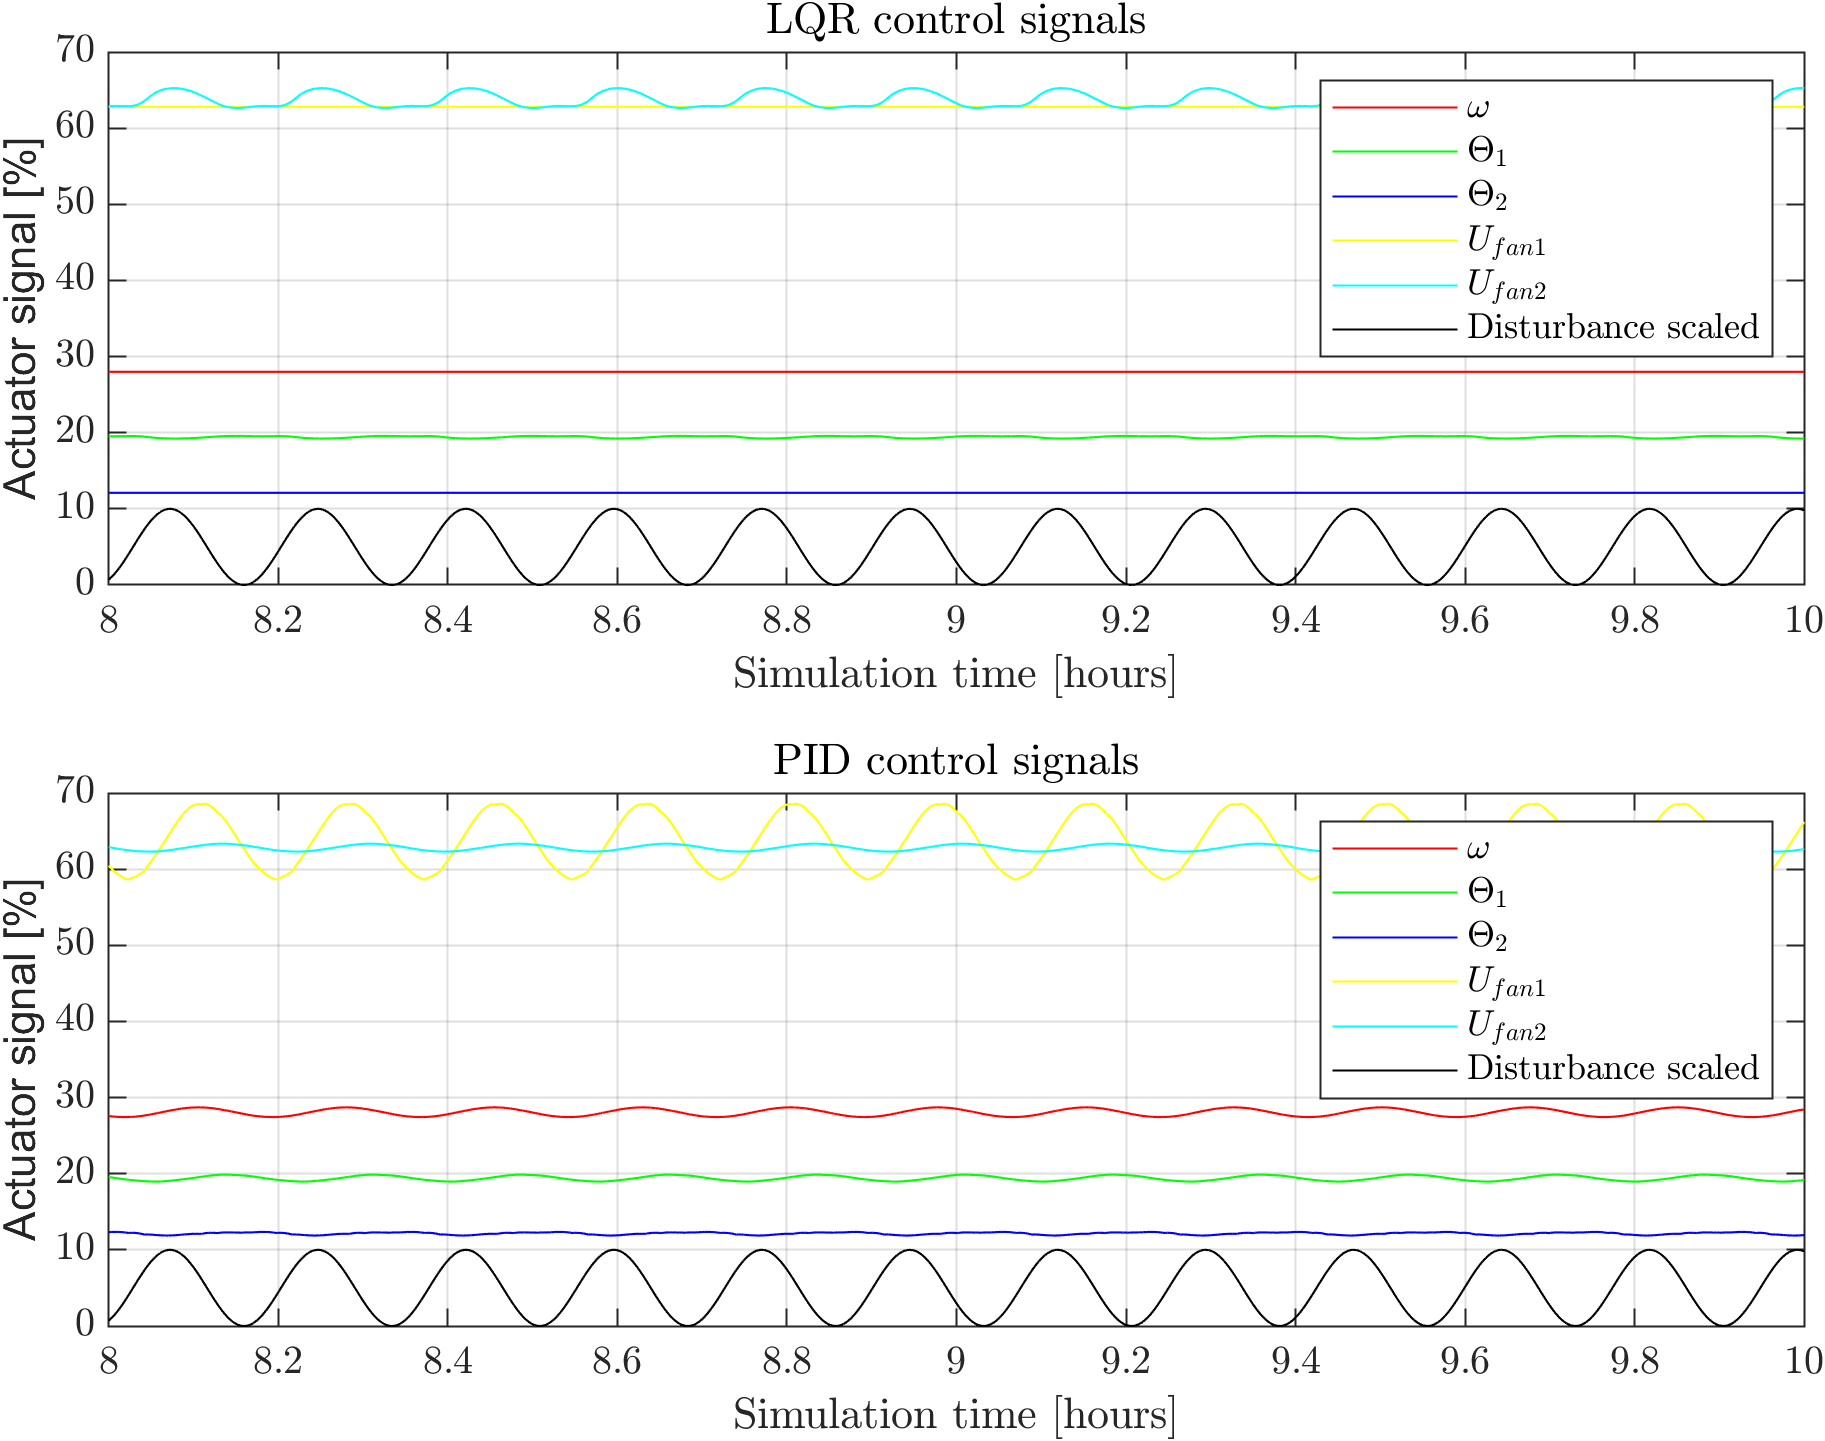
\includegraphics[width=0.71\textwidth]{Graphics/fig_inputs_sineDist_zoom.png}
	\caption{Zoomed version of \cref{fig:inputs_sineDist}. Sine disturbance case: Plot of the control signals applied to the Hi-Fi Simulation (zoomed). Top: LQR control signals. Bottom: Hi-Fi simulation PID control signals. Note that the PID controller affects all control inputs and the OBLQR controller only affects two.}
	\label{fig:inputs_sineDist_zoom}
\end{figure}

As mentioned, the PID controller varies all control signals to mitigate the sine disturbance, whereas the OBLQR can only make use of control signals $ \Theta_1 $ and $ U_{fan2} $. As the PID controller seem to have a better performance than the OBLQR in terms of oscillations in controlled outputs, a last measure of performance is investigated, namely the power consumption.  
The average power consumption in the time interval from 9-10 hours is 1.68 \si{kW} for the OBLQR compared with 1.67 \si{kW} for the PID controller. The energy consumption throughout the two parallel simulation runs are respectively 25.32 for the OBLQR and 25.21 \si{kWh} for the PID controller. This means that the OBLQR is slightly less energy efficient than the PID controller. Again, the model mismatched is assumed to be the cause that the performance could not be improved with the OBLQR.

\subsection{Tuned OBLQR controller: Step disturbance}
To test the models ability to continuously perform outside the operating point, a step disturbance is applied to the ambient temperature.  At time $t=3$ hours, a 5$^{\circ}$C step in the disturbance is introduced. This implies that the ambient temperature initially is 20$^{\circ}$C and after the step is 25$^{\circ}$C. As before the PID structure handles the first hour of simulation, after which the OBLQR controller takes action. The controlled outputs are seen in \cref{fig:LQR_wellTuned_5stepDist}.
\begin{figure}[H]
	\centering
	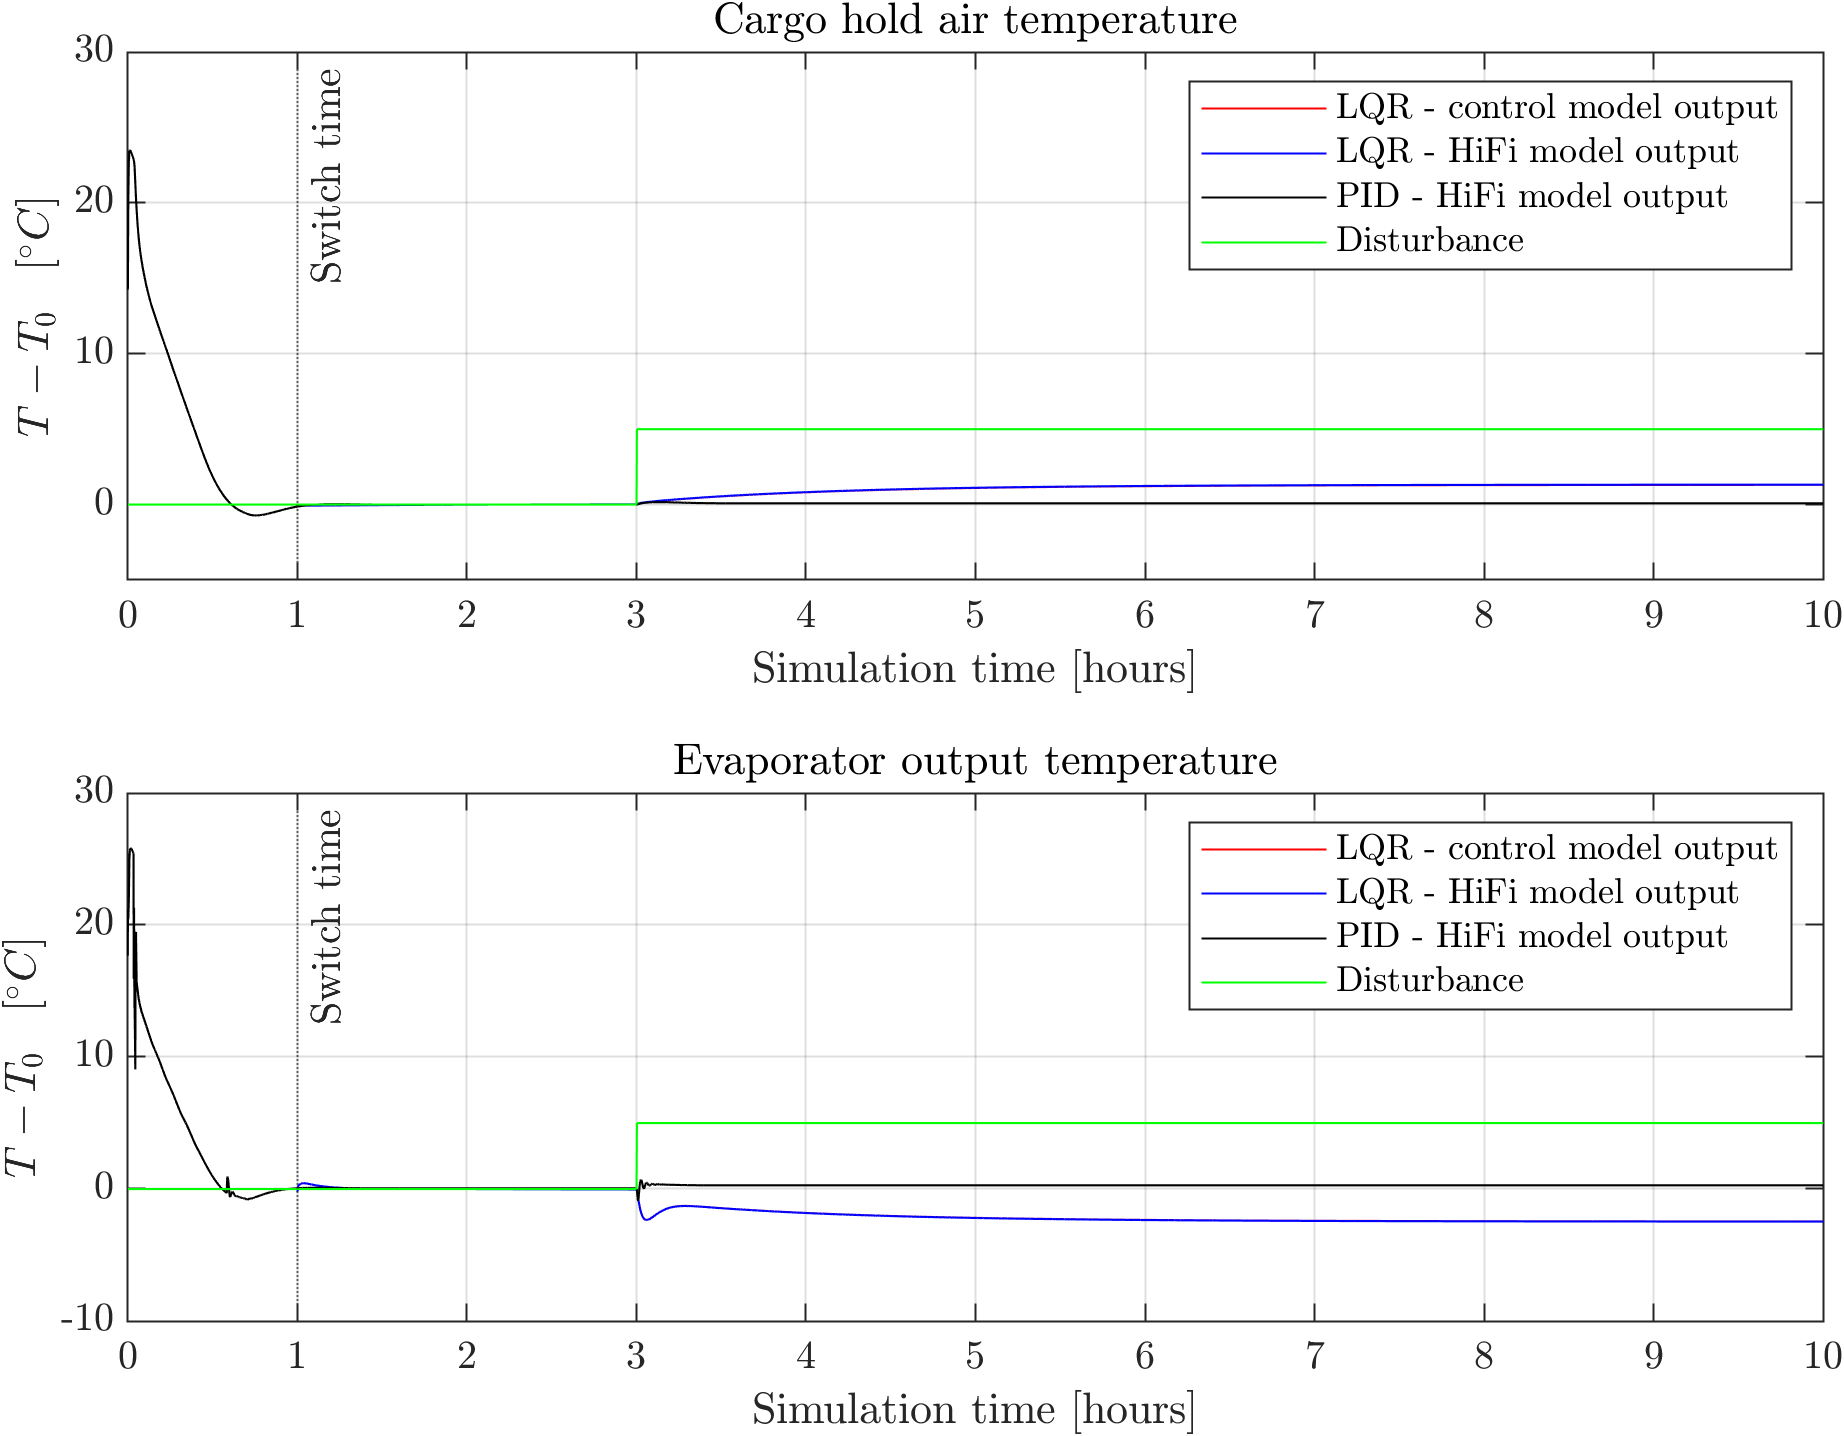
\includegraphics[width=1\textwidth]{Graphics/fig_LQRvsKresten_stepDist.png}
	\caption{Step disturbance case: Top: Cargo hold air temperature. $T_0$ = -4.25$^{\circ}$C. Bottom: Evaporator vapor refridgerant temperature. $T_0$ = -5.55$^{\circ}$C}
	\label{fig:LQR_wellTuned_5stepDist}
\end{figure}
From inspecting the steady state error of the two control strategies in \cref{fig:LQR_wellTuned_5stepDist}, it is apparent that the PID controller has a much smaller steady state error for both the cargo hold temperature and evaporator output temperature. A closer investigation of the output response is seen in
\cref{fig:LQR_wellTuned_5stepDist_zoom}. 

\begin{figure}[H]
	\centering
	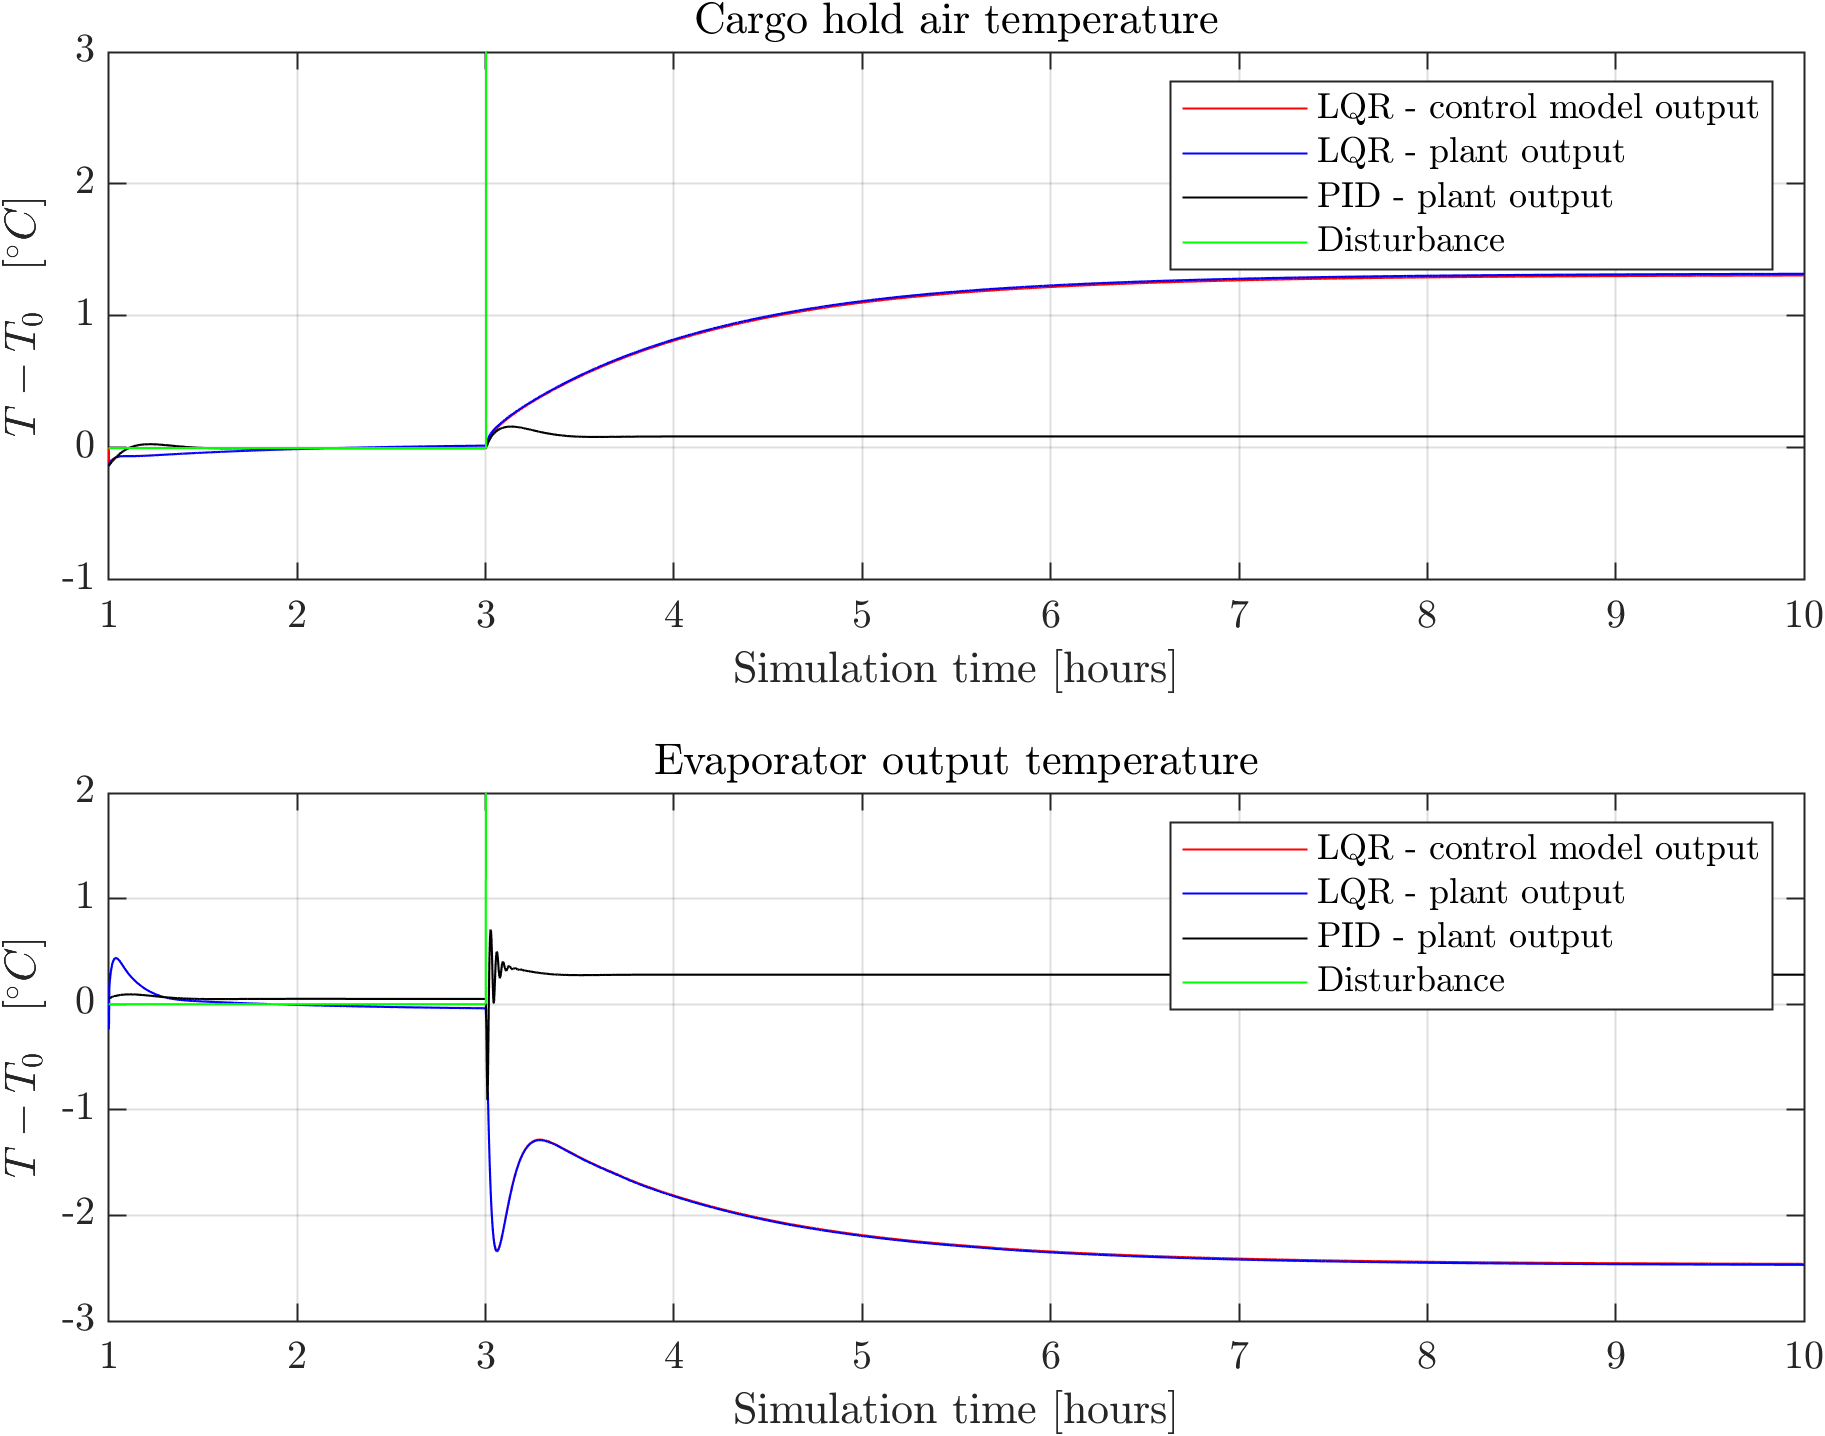
\includegraphics[width=1\textwidth]{Graphics/fig_LQRvsKresten_stepDist_zoom.png}
	\caption{Zoomed version of ,\cref{fig:LQR_wellTuned_5stepDist}. Step disturbance case: Top: Cargo hold air temperature. $T_0$ = -4.25$^{\circ}$C. Bottom: Evaporator vapor refrigerant temperature. $T_0$ = -5.55$^{\circ}$C}
	\label{fig:LQR_wellTuned_5stepDist_zoom}
\end{figure}

\noindent In subplot 1 it is seen that the cargo hold air temperature converges to 1.25$^{\circ}$C above the operating point for the OBLQR, whereas for the PID controller it converges to less than 0.1$^{\circ}$C above the operating point.
For the OBLQR it means $T_{air} = -3^{\circ}C$, compared with an operating point of 4.25$^{\circ}C$
The transient response of the PID controller is much faster than that of the OBLQR, which is desirable. 
Inspecting subplot 2, the evaporator output temperature for the OBLQR drops to -2.4$^{\circ}$C below the operating point, which means there is 3.6$^{\circ}$C superheat. The PID controller output temperature increases to about 0.25 $^{\circ}$C above the operating point.
However, the PID controller overshoot and the amounts of oscillations could indicate that it is closer to instability than the OBLQR.\\

The increase in air temperature is large enough to be considered a problem for transportation of temperature critical goods, which is of course the intended purpose of the reefer trailer. The cause of this is likely, as was the case for the sine disturbance, that the controller is unable to change the compressor speed. The compressor speed and expansion valve opening degree is critical for increasing the refrigerant flow through the refrigeration circuit, and is thus highly correlated with the cooling capacity of the system. \\

The drop in superheat is not as critical a problem as the air temperature. Ideally the controller would be able to keep it at the operating point, and in that context it is not desirable behavior. Technically, a drop in superheat increases the evaporation efficiency, and as long as there is a positive superheat no liquid will flow into the compressor. In summary, while the drop in superheat might increase efficiency without damaging the compressor, it would be a far more appealing if the controller was able to maintain the superheat at a fixed value.

The control inputs during this test is seen in \cref{fig:inputs_stepDist}.

\begin{figure}[H]
	\centering
	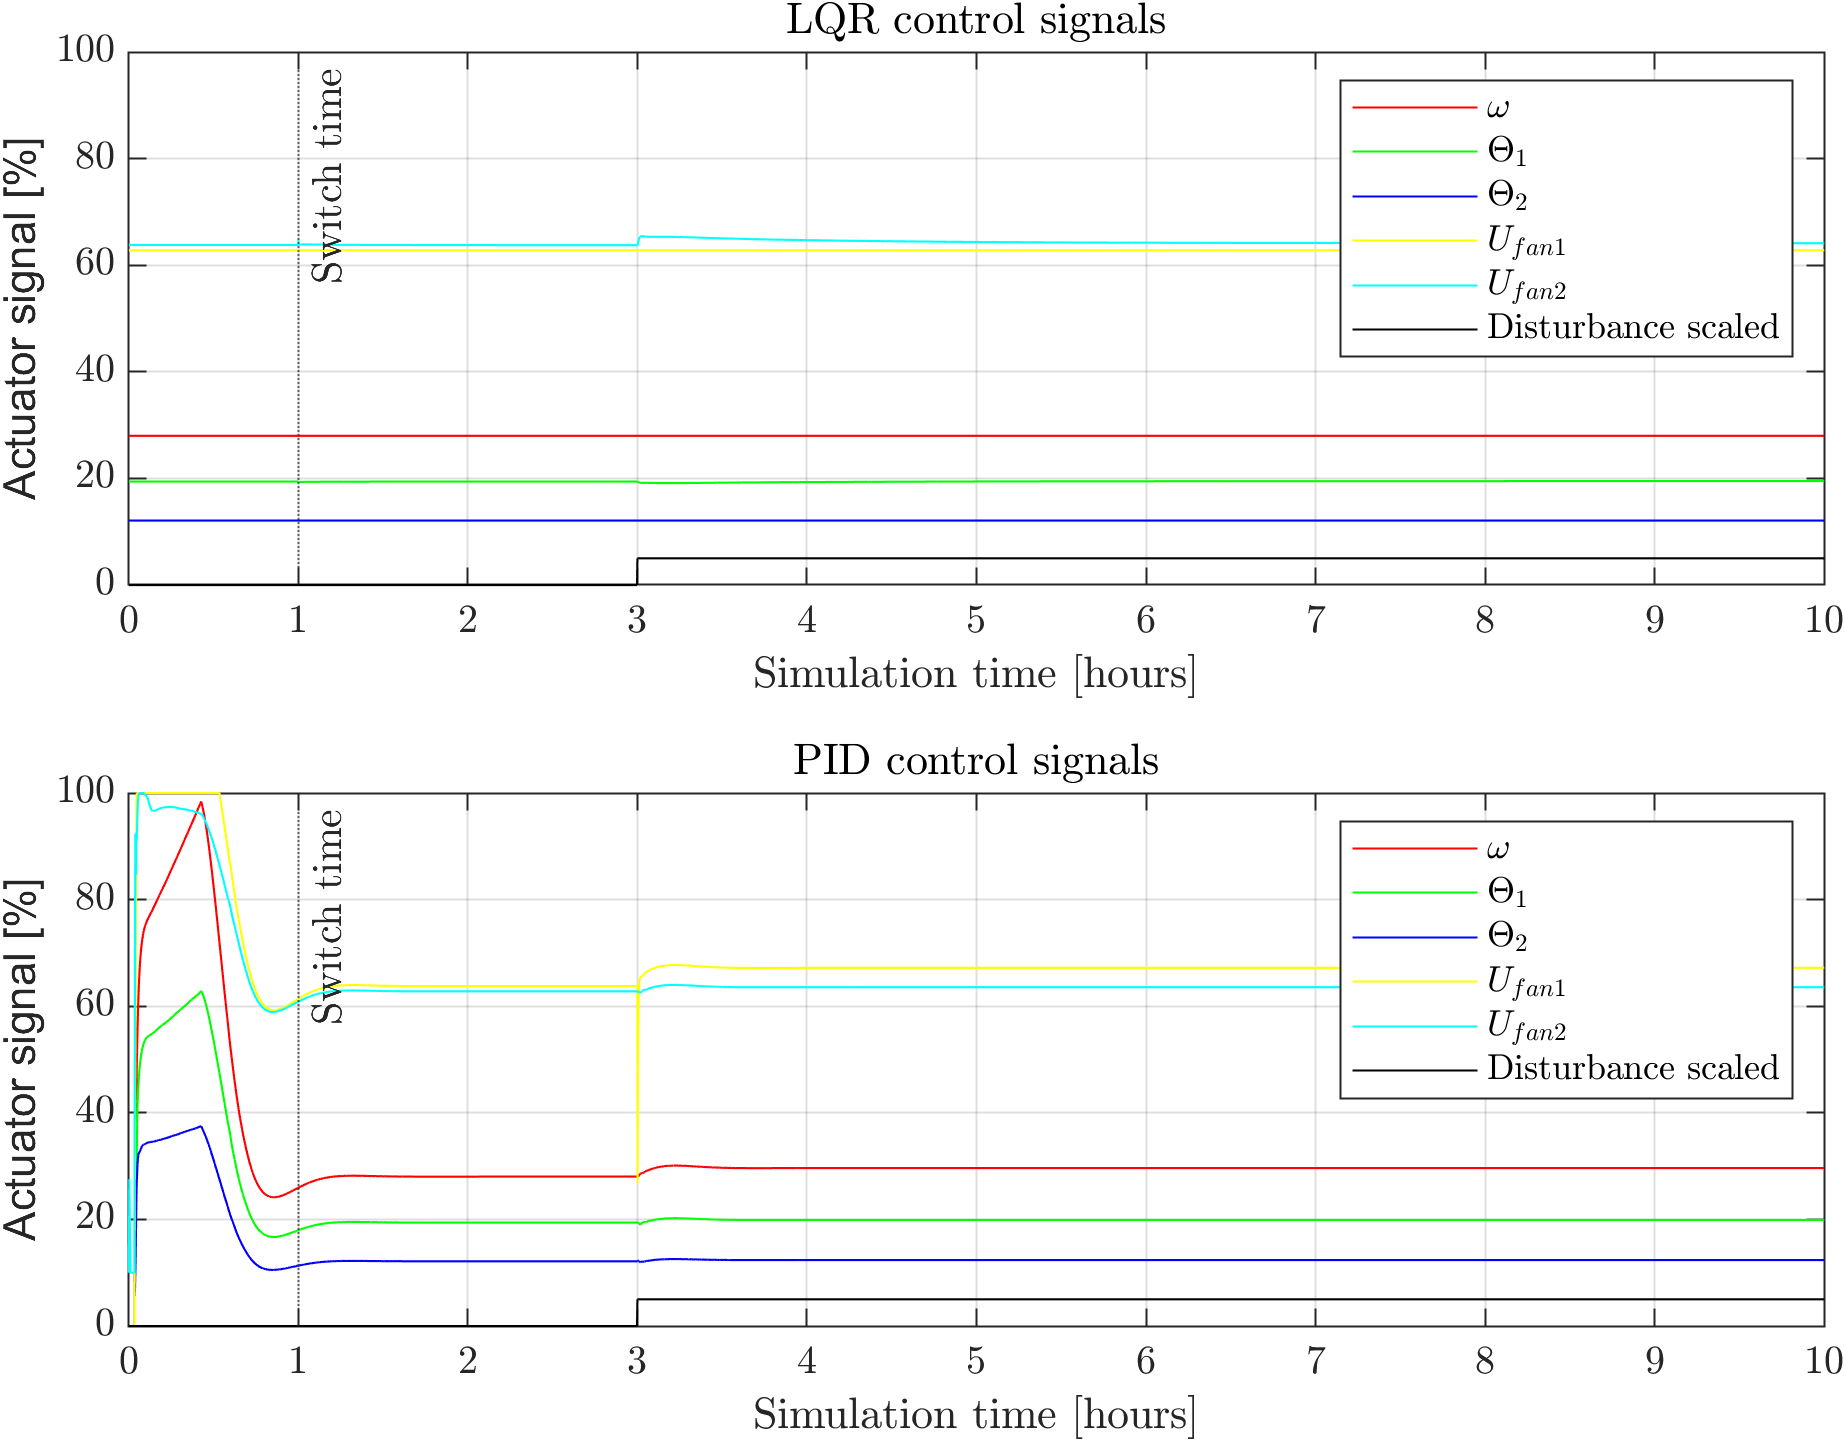
\includegraphics[width=1\textwidth]{Graphics/fig_inputs_stepDist.png}
	\caption{Step disturbance case: Plot of the control signals applied to the Hi-Fi Simulation. Top: LQR control signals. Bottom: Hi-Fi simulation PID control signals.}
	\label{fig:inputs_stepDist}
\end{figure}

As expected, the OBLQR controller only affects the two inputs it has acces to, namely $ \Theta_1 $ and $ U_{fan2} $, whereas the PID controller affects all control signals. However all control signals are in a valid range for the actuators.
The last measure to conclude upon is the power consumption of the two controllers. The power consumption in steady state for the OBLQR is 2.02 \si{kWh} compared with 2.06 \si{kWh} for the PID controller. The total energy consumption during the parallel simulation runs are respectively 28.99 \si{kWh} and 29.46 \si{kWh} for the OBLQR and PID controller.
This is the only test case where the OBLQR proves to have lower power usage than the PID controller. However, the lower power consumption comes with the price of a higher steady state error, and it can thus not be considered a better controller, as the cargo temperature is the main objective, and the power consumption is the secondary objective. 

\subsection{Test Conclusion}
The OBLQR controller is able to stabilise the system for all three test cases where it is initiated near the operating point. This includes a sine disturbance with amplitude of 5 $ ^{\circ} $C and a step disturbance of 5 $ ^{\circ} $C. The stabilisation is obtained with valid inputs. The OBLQR generally obtains similar performance to the PID controller, with similar control inputs. This is likely directly linked to the fact that the operating point for the linearised model is obtained with the steady state control inputs of the PID controller.
Even though the control performance is similar there are some drawbacks that is in the PID controllers favor. The OBLQR controller has slower transient response than the PID controller. It also has greater steady state errors that the PID controller. 
In addition, the power consumptions of the two are also very similar, with no significant improvements for the OBLQR compared with the PID controller.
The model accuracy is assumed to be the major bottleneck as to obtain improved controller performance for the OBLQR compared with the PID controller.